\renewcommand{\inputfile}{\version\ - edited 2008-06-26 flotsam}
% $Author$ $Date$
%
% Predrag moved from blog/ to thesis/chapters/  jun 26 2008
% Predrag created file                          jun 20 2006

Squirreled away for the thesis from material omitted form the KS papers.
Predrag moved the material here from blog/flotsam.tex on June 26 2008.

\section{Squirreled away for the next KS paper}
% from energy.tex

{\bf PC}: believe it or not, we are now set to compute
    $\timeAver{E}$ and $\timeAver{P}$
    using cycle expansions


Substitution by \refeq{KSeqvCond}
verifies that for an \eqv\ $\expctE$ is constant:
\[
   \dot{\expctE} =
\expct{ \left({u^2}/{2} + u_{x} + u_{xxx} \right) u_x}
    = \expctE \expct{ u_x }=0
    \,.
\]


% PC worked out in part with Bridges
An infinite number of identities for moments of
solutions of KS follow\rf{Bridges_priv}. For example,
integrating by parts $\expct{u_{x} u_t}$,
$\expct{u_{xx} u_t}$,
and
$\expct{u^2 u_t}$,
respectively, one obtains \reqva\ relations
\PC{please re-derive these three. Are there more
    important ones that I have missed?
    Also, I - unnecessarily - specialized to \reqva,
    but these identities will be especially useful for \rpo s}
\RLD{I don't quite follow this process of deriving moments.  What is
the reason we look for some combinations of $u$ and its derivatives?
Why not just take $\expct{u_{x\cdots x}}$?
Is there any physical motivation for such combinations,
beyond $E$, $P$ and $D$?  Maybe use things like $\dot{P}$,
$\dot{D}$, etc.?}
\PC{they merit more thought and time than we have now, so let's
   pick them up after the first paper is submitted}
\bea
% \expct{u_{x} u_t}
%     \qquad \to \qquad
c P &=& \expct{u \, u_{x}{}^2}
\label{Bridges1}\\
c P  &=& \expct{u \, u_{xx}{}^2}
\label{Bridges3}
\,.
\eea
True for any solution:
\bea
% \expct{u_{xx} u_t}
%     \qquad \to \qquad
\dot{P} &=& 2P - \expct{u_{x}{}^3}  - 2 \expct{u_{xxx}{}^2}
\label{PC1}\\
\dot{D} &=& 2\expct{u_{xxxx}{}^2}
    + 5 \expct{u_{xx}{}^2 u_{x}}  - 2 \expct{u_{xxx}{}^2}
\label{PC2} \\
\dot{P} &=& 2P - \expct{u_{x}{}^3}  - 2 \expct{u_{xxx}{}^2}
\label{PC3}\\
\frac{d^2 E}{dt^2} &=& \dot{P} - \dot{D} =
     2P - \expct{u_{x}{}^3}
    - 2\expct{u_{xxxx}{}^2} - 5 \expct{u_{xx}{}^2 u_{x}}
\label{PC4}\\
\frac{d}{dt} \expct{u_{x}{}^3} &=&
        3 \expct{u_{x}{}^3u + u_{xx}{}^3}
\label{PC5}
\,.
\eea
When moments such as \refeq{Bridges1} are added as
coordinate axes to \reffig{f:drivedragConn}, \reqva\ and
\rpo s are separated from \eqva\ and \po s. Furthermore,
as higher moments have more and more powers of $u$ and derivatives
$u_{xx\cdots x}$, their magnitudes should be strongly suppressed,
providing a symmetry-invariant basis set that can be safely truncated to
a finite-dimensional \statesp.
See  \refsect{sec:energyL22} for how this works out in practice.


%%%%%%%%%%%%%%%%%%%%%%%%%%%%%%%%%%%%%%%%%%%%%%%%%%%%%%%%%%%%%%%%
\begin{figure}[t] \label{f:drivedragPoinc}
\begin{center}
    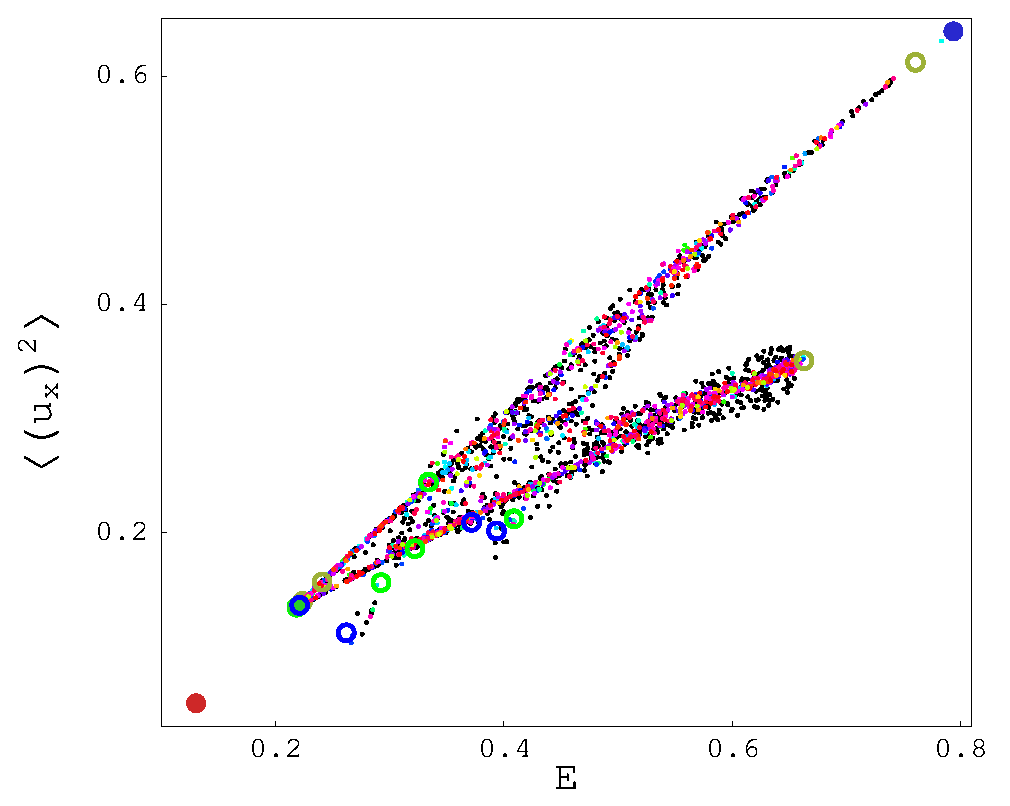
\includegraphics[width=0.8\textwidth]{../figs/energyPoinc}
\end{center}
\caption[Poincar\'{e} surface of section for L=22]
        {
Shown on Poincar\'{e} surface of section
$\expct{(u_{xx})^2} = \expct{(u_{x})^2}$:
\EQV{1}, \EQV{2} and \EQV{3} in red, green and blue solid points respectively,
connections from \EQV{1} to $A(L/4)\EQV{1}$,
from $A(L/4)\EQV{1}$ to \EQV{1} and from \EQV{3} to $A(L/4)\EQV{1}$ in green,
yellow-green and blue circles respectively,
a typical ``turbulent" evolution (black) and all \po s and \rpo s
determined so far for $L=22$.
        }
\end{figure}
%%%%%%%%%%%%%%%%%%%%%%%%%%%%%%%%%%%%%%%%%%%%%%%%%%%%%%%%%%%%%%%%%%

\PCedit{PC: Poincar\'{e} surface of section \reffig{f:drivedragPoinc}
probably does not make sense - the motions of various magnitudes squared,
are only shadows of the true dynamics in the full \statesp. Being close here
does not mean that one is close in the \statesp\ - only point that are
distant from each other here have to be also distant in the full space.
       }

 \RLDedit{with small subsets of
symmetric (eventually) \po s lying on $d=0$, $d=L/2$, \etc\ lines.}
\RLD{All orbits we found with $d = 0$ have reflection symmetry,
so they are discussed later as \po s.  We found no orbits with
$d = L/m$ exactly, so the highlighted statement needs to be dropped or
modified somehow.}
%\PC{\reffig{f:ks22rposT} needs $\Delta\to \shift$. If you document the
%   figure source codes, any one of us can edit figures, nein?. }

 It is the unstable manifold of the \EQV{2}
{\eqv}, drawn by tracing out a set of points along one of the complex
eigenvectors, that start close to it. Surprisingly, everybody connects
to the \EQV{2} shifts by 1/2 wavelength ($d = L/4$) but as we are in
$\infty$-dimensions they do it not as the usual homoclinic connection, but in
many (all?) possible intermediate ways. This might be a clue for how to
partition symbolic dynamics.
What is great about
this is that the \EQV{2} unstable manifold has a heteroclinic connection to itself
$L/2$ shifted, but
even better, to \EQV{2}, and \EQV{3} unstable manifold has a heteroclinic
connection to \EQV{2}.
% It's really pretty.
That makes for a rigid backbone -
we hope this will help us develop a symbolic dynamics for \rpo s.

The KS work
% described in \refsect{s:KS}
of \refref{Christiansen:97}
was restricted to the antisymmetric subspace.
The restriction to antisymmetric subspace was used
to eliminate the continuous translational symmetry of \KSe.
Due to the lack of self-adjointness
(non-normality) of the linearized \KS\ flow,
the antisymmetric subspace
is unstable under small perturbations, and generic solutions of
KS belong to the full, periodic space.
Nevertheless,
the \eqva\ and the shortest \po s orbits that lie in this subspace
and play important role for global topology of the flow,
together
with the \reqva\ and \rpo s
characteristic of the full, continuous translation invariant space..

%%%%%%%%%%%%%%%%%%%%%%%%%%%%%%%%%%%%%%%%%%%%%%%%%%%%%%%%%%%%%%%%
% former {figure}[t] \label{f:KS22cage}
\begin{figure} [t]
\begin{center}
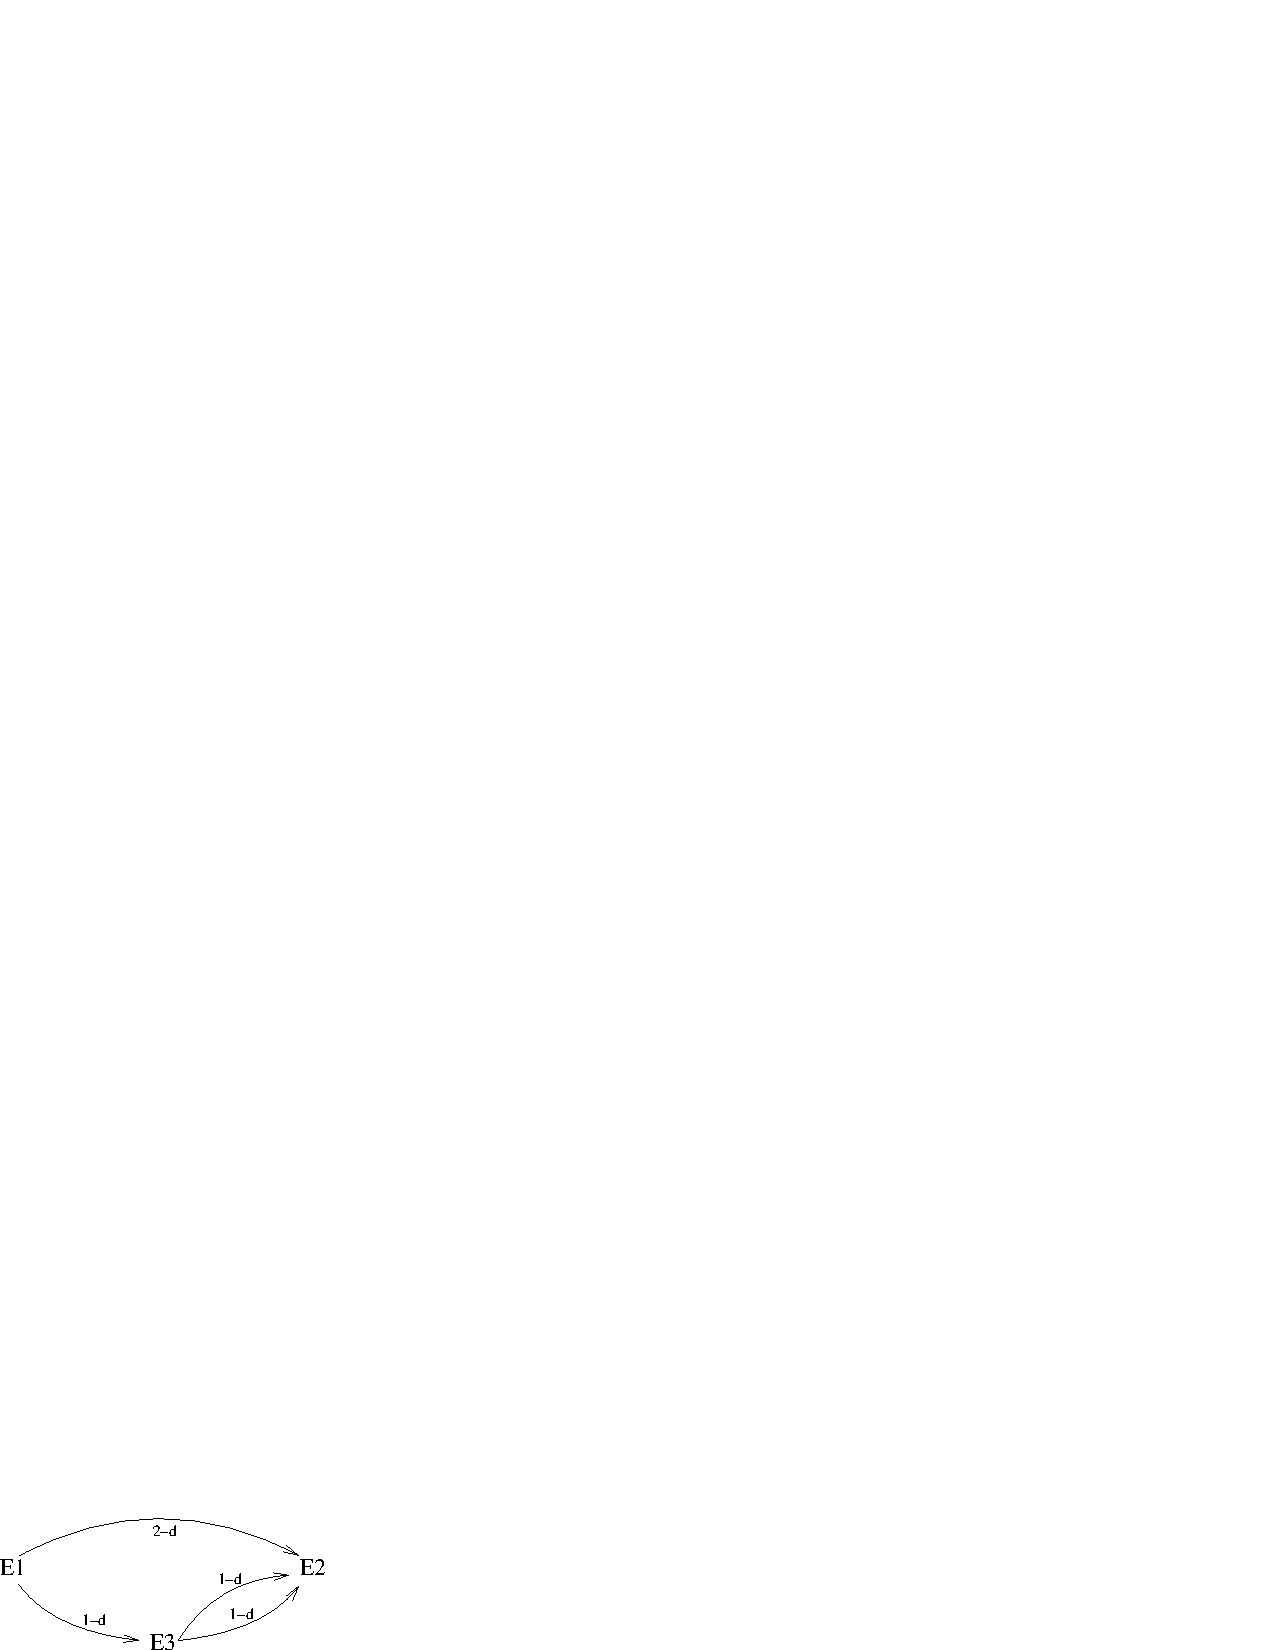
\includegraphics[width=0.3\textwidth]{../figs/ks22_E1_UM_diag}
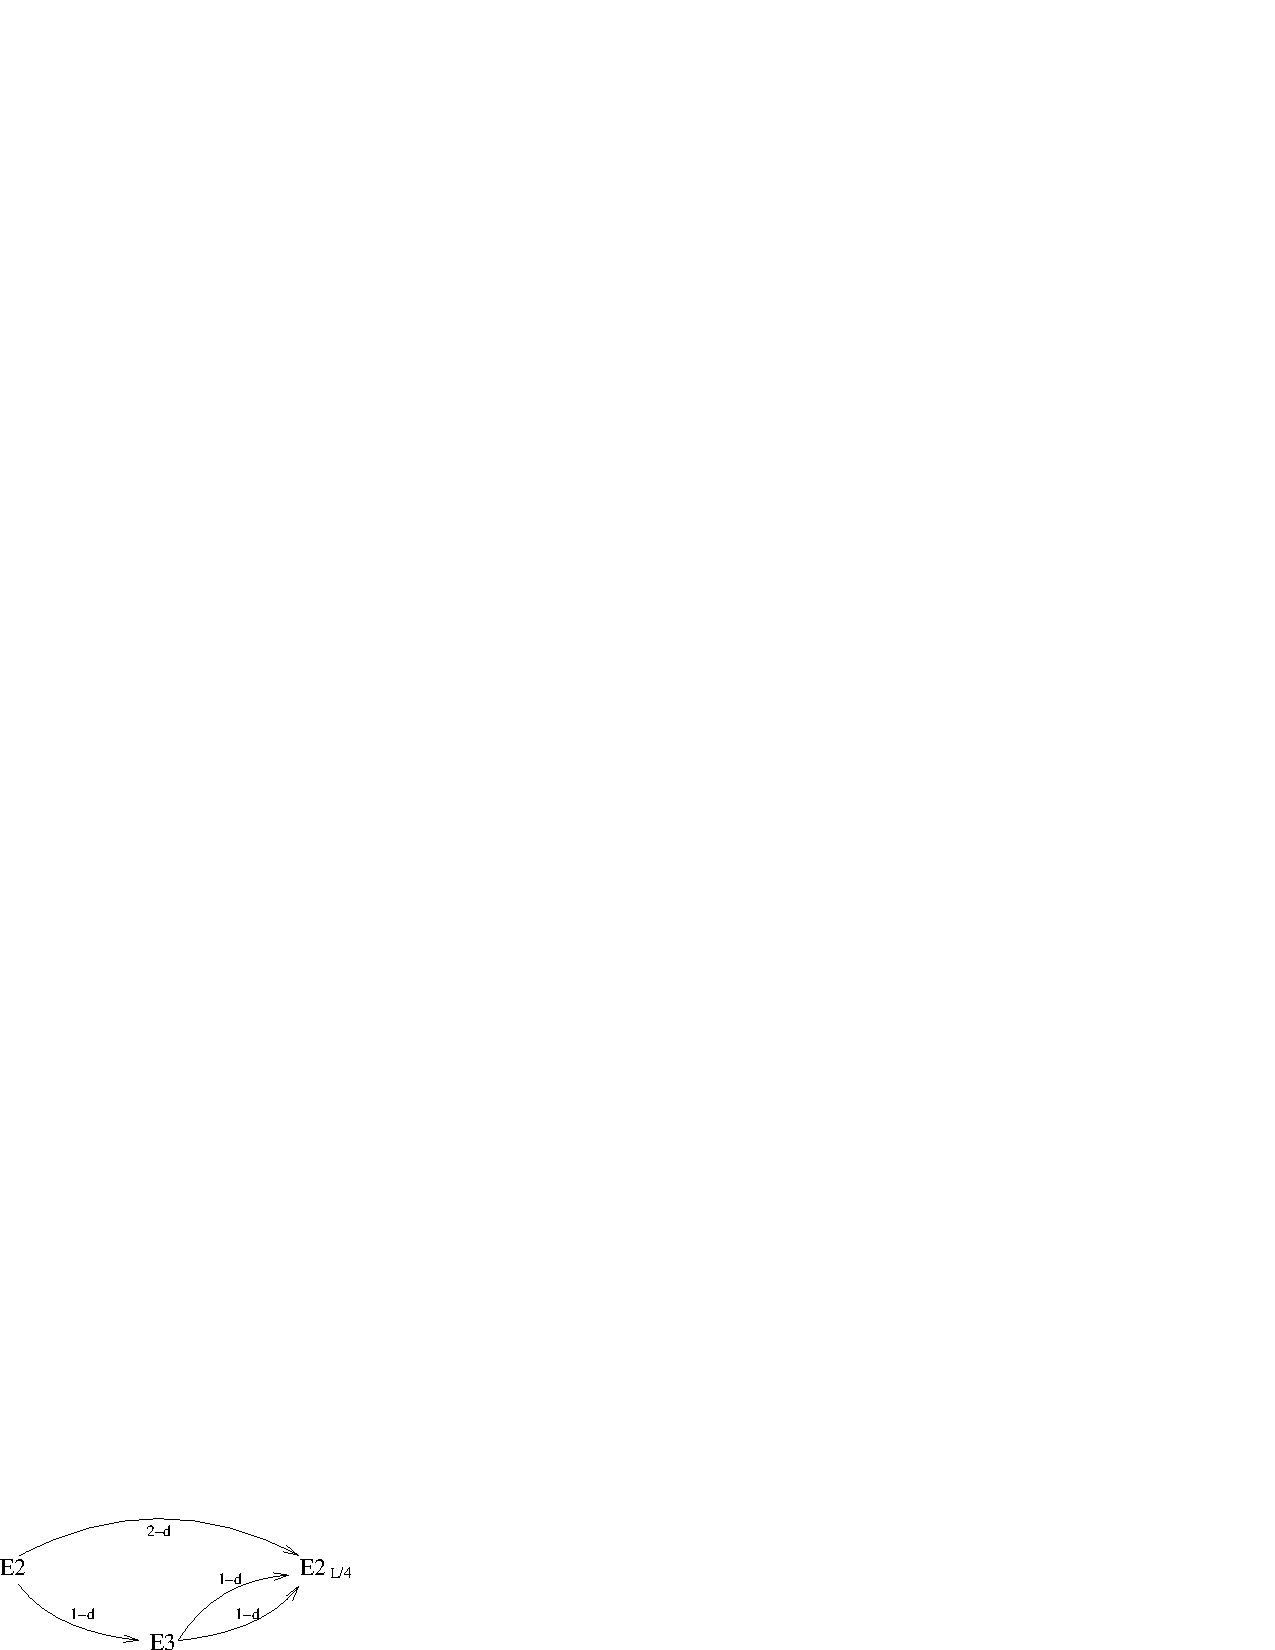
\includegraphics[width=0.3\textwidth]{../figs/ks22_E2_UM_diag}
\end{center}
\caption[OBSOLETE: EQV{1}~\eqv\ unstable manifold]
        {OBSOLETE:
\EQV{1}~\eqv\ unstable manifold,
    with the trajectory connecting the
\EQV{2}~\eqv\ point to the unique corresponding heteroclinic
point in the \EQV{3}~\eqv\ family.
\EQV{3}~unstable manifold in turn connects \EQV{3} to the
stable manifold of \EQV{2}.
  %
\PCedit{
Edit the cage of heteroclinic connections,
xfig file /rpo\_ks/figs/ks22\_E1\_UM\_diag.fig
and rpo\_ks/figs/ks22\_E2\_UM\_diag.fig
    }
        }
\label{f:KS22cage}
\end{figure}
%%%%%%%%%%%%%%%%%%%%%%%%%%%%%%%%%%%%%%%%%%%%%%%%%%%%%%%%%%%%%%%%%%
{\bf PC}: a bit of a cheat - \reffig{f:KS22unstM} has
    2 unstable complex-pair planes

rescue the nice heteroclinic connection figure
    in \reffig{f:KS22unstM}\,(\textit{b})

    \refFig{f:KS22unstM} move (a) to flotsam

{\bf RLD:} I have the feeling that it can be proven that there are
no other types of symmetries that lead to exactly periodic
solutions, but I don't know how to construct such a proof.
%In the first case the whole orbit lives within the antisymmetric subspace.

{\bf PC}: show what happens to \eqva\ of \eqva\ eigenvalues
\refeq{eqvEqvEigV}
as $E \to $ large.

\bigskip

As a result, KS can have
%\reqva\ (traveling wave) solutions $u(x-ct)$ and
\rpo\ $p$ with period $\period{p}$ and
a nonzero shift $\shift_p$
\beq
%\tau_p \Refl_p u_p(x,0) =
\sigma_p u_p(\sigma_p x+\shift_p,\period{p}) = u_p(x,0)
\,,\qquad
\sigma_p \in \{+1,-1\}
\,,
\ee{KSrposFlot}
\ie, a state $u_p(x,0)$ that occurs again after time $\period{p}$,
but shifted by $\shift_p$, and possibly reflected by $\Refl$.
{\Rpo s} are periodic in $c=\shift_p/\period{p}$
co-rotating frame,
but in the stationary frame their trajectories
are quasiperiodic.
Due to the reflection symmetry \refeq{KSparity} of KS equation,
every \rpo\
$u_p(x,t)$ with shift $\shift_p$ has a symmetric partner
$-u_p(-x,t)$ with shift $-\shift_p$.

%
{\bf PC}:
 % Past: Michael Loss has not taught us how to bound $E$ by
 %  Sobolev bounds. Neither has Spiegel. Next: But
  Constantin says that the answer is in
    \refrefs{temam85ks}. Eckmann says: the  best bound is by Otto\rf{GiacoOtto05}; the
    only bound close to k=0, better in essential way. See also \refref{bronski-2005}.
    Eckmann had $L^{8/5}$, but conceptually Otto is the best. Recheck whether it is
    $|u|$ or $E \propto L^{3/2}$.
    When the solution is big, how long can it stay big? They found it cannot stay big for
    long.


from bounds on energy, we might be able
to bound the number of \eqva\ as function of systems size $L$, and thus
be sure we have them all.

Next for you guys: read Lieb and Ruelle to learn
    how to bound $E$  by Sobolev bounds.

\subsection{Template for KS equilibria discussion}

Ruslan L. Davidchack 3 Sep 2006:
http://www.math.le.ac.uk/people/rld8/temp/kse22explore.html homepage.


ES:{I observe pairs of real eigenvalues,
e.g. -58.3602685 and -58.3602681. As their absolute
value increases they differ even less.
I think it has to do with the linear part being the main
contribution to $\Mvar$ for higher modes, as well as
with treating real and imaginary components
as separate variables, which means it will appear twice.
        }

PC: {I think such contracting eigenvalues as -58.3602685 have no meaning.
Even if they are accurate eigenvalues of $\Mvar$,
what use is
$\ExpaEig_{radial} =  e^{\Lyap_p \period{p}} = e^{26\cdot58} = e^{1510}$.
        }

The \reqva\ (or traveling waves) appear to have a limiting propagation
velocity $c_{max} = \pm d/\period{}$.
To visualize them numerically,
start with a localized self-dual $u(x,0)$ such as
\[
u(x,0) = x e^{- x^2/2\sigma^2}
\,,
\]
with typical width $\sigma/2$ of order of typical wavelength
$\sqrt{2}$ (in $\tilde{L}$ system size units).
Time evolution of this  $u(x,t)$ is bracketed by two constant
pulses of apparently constant velocity $v=?$.
\RLD{generate figure, state $\sigma/2$, estimate $v$}
The notion of ``velocity''
is fuzzed up by the fact that the large peaks are preceded
by smaller precursors.

PC: {Determine their velocity ANALYTICALLY?}

consult often
\\
        www.math.le.ac.uk/people/rld8/temp/kse22explore.html
\\
we have to systematize it, and
construct the complete cage of heteroclinic $\EQV{1}$, $\EQV{2}$, $\EQV{3}$,
$\REQV{+}{1}$,
$\REQV{-}{1}$,(?)
connections, \underline{divided} by the $u(x) \to - u(-x)$ symmetry.

The hope is that $\EQV{1}$,
$\REQV{+}{1}$,
$\REQV{-}{1}$,(?) are transient, and \rpo\ symbolic
dynamics (\underline{divided} by the $u(x) \to - u(-x)$ symmetry, otherwise
unnecessarily messy) comes from the closed loops on
the $\EQV{2}$,$\EQV{3}$ part of the cage.



\example{Stability of \KS\ equilibria:}{
% \label{exam:KSEquilStab}
% \index{Kuramoto-Sivashinsky equilibria}
\begin{table}
\caption[Important \KS\ equilibria]{
Important \KS\ equilibria:
% in the antisymmetric solution
% space of the Kuramoto-Sivashinsky equation with periodic boundary % % % % condition,
% $ \nu =1$, $L=38.5$;
% their labels,
the first few stability exponents
%, with complex pairs written together.
}
\begin{center} \footnotesize
\begin{tabular}{@{}ccccc}
\hline %\br
$~S~~~$ & $~~~~\lambda_1 \pm \,i\,\theta_1$
                                & $~~~~\lambda_2 \pm \,i\,\theta_2$
                                        & $~~~~\lambda_3 \pm \,i\,\theta_3$
\\
\hline %\mr
${C_1}$    &{0.04422 $\pm \,i\,$0.26160}   &-0.255 $\pm \,i\,$0.431
&-0.347 $\pm \,i\,$0.463         \\
% ${C_2}$    &0.33053  & 0.097 $\pm \,i\,$0.243
% &-0.101 $\pm \,i\,$0.233        \\
\hline %\mr
${R_1}$   &{0.01135 $\pm \,i\,$0.79651} & -0.215 $\pm \,i\,$0.549
&-0.358 $\pm \,i\,$0.262        \\
%  ${R_2}$   &  0.33223  & -0.001 $\pm \,i\,$0.703
%  & -0.281 $\pm \,i\,$0.399      \\
\hline %\mr
${T}$     & 0.25480  & -0.07 $\pm \,i\,$0.645 &-0.264
\\
\hline %\br
\end{tabular}
\end{center}
\label{t:stationary}
\end{table}

{\em
spiraling out in a plane}, all other directions contracting


{\bf
Stability of ``center'' equilibrium
    }

linearized stability exponents:
\[ % \beq
(\lambda_{1}\pm\,i\,\theta_{1},\lambda_{2} \pm\,i\,\theta_{2}, \cdots)
    = (0.044 \pm \,i\,0.262\,,\,
        -0.255 \pm \,i\,0.431\,,\,\cdots)
\] %\eeq

The plane spanned by $\lambda_{1} \pm\,i\,\theta_{1}$ eigenvectors rotates with angular period
$\period{} ~\approx~2\pi/\theta_{1}=24.02$.
% 2*4*a(1)/0.26160 = 24.0182924586375

a trajectory
that starts near  the $C_1$~equilibrium point spirals
away per one rotation
with multiplier
$\ExpaEig_{\mbox{radial}}~\approx~\exp(\lambda_{1}\period{})=2.9$.
% 2*4*a(1)/0.26160*0.04422 = 1.062
% e(1.0620888) = 2.8924063421

each Poincar\' e section return,
contracted into the stable manifold by
factor of
{
$\ExpaEig_{2}\approx\exp(\lambda_{2}\period{})=0.002$
}
%2*4*a(1)/0.26160*(-0.255) = -6.12466
%e(-6.12) = .0022


The local Poincar\' e return map is
{\em
in practice $1-dimensional$
}
    } %end \example{{Stability \KS\ equilibria


Staring at the solution
 as it evolves in time we should start getting a glimpse of the
 repertoire of the spatiotemporal patterns characterizing
 the turbulent dynamics.

Many of the \rpo s can be constructed from segments corresponding to
close approaches to some of these \eqva.

\textbf{ES}: Greene and Kim show that steady states (non-traveling)
have to be antisymmetric and our findings verify it.

\textbf{PC}: do they really show that? I think they must be symmetric under both
{\Refl} and \Shift, otherwise they could be invariant under one,
but traveling, not invariant under the other one.

\textbf{ES}: They provide an argument for this which did not yet convinced me.
\EQV{2,3} are symmetric under both {\Refl} and \Shift, \EQV{1} is not
symmetric under \Shift, but when I say traveling I mean traveling waves,
this does not refer to behavior under symmetry.

If Greene and Kim
are correct we would get the same equilibria for both
antisymmetric and full space. If equilibria provide the coarsest organization
of \statesp\ then we should expect characteristic orbits for $L=22.0$
for full space and $L=44.0$ for antisymmetric subspace to be completely different.
Of course for $L=22.0$ the full space dynamics will be richer than
in the
antisymmetric subspace, but I don't think this can be quantified by
dividing $\tildeL$ by $2$.

\textbf{PC}: you are right.


\subsection{Numerical methods}

Shroff and Keller\rf{shroff:1099}
``The Recursive Projection Method" (RPM)
might be of interest to us in numerical work.
RPM stabilizes fixed-point iterative
procedures by computing a projection onto the unstable subspace.
On this subspace a Newton or special Newton iteration is performed,
and the fixed-point iteration is used on the complement.
The method is effective when the dimension of the unstable subspace
is small compared to the dimension of the system.
Examples are presented for computing unstable steady states.
The RPM can also be used to accelerate iterative procedures when
slow convergence is due to a few slowly decaying modes.

PC also has 2 hard-copy, rather readable
old proceedings reprints by Keller\rf{Keller77,Keller79}.
There are some readable words about homotopy methods in
\refref{AllgGeorg88}.

{\Rpo s} were missed in earlier
previous \KS\ investigations%
\rf{Christiansen:97,Lan:Thesis}
which focused on the antisymmetric subspace, where translational invariance
is broken.

%% Davidchack and Crofts
 We investigate this system in 16 to 64 complex Fourier modes (32 to
128-dimensional system of real ODEs) truncation, and recheck the results
by redoing the calculation with the double number of Fourier modes. %
observe how many digits change. The \eqv\ points are accurate to at least
to $10^{-11}$. Since Lapack is also double precision accurate, the
accuracy of the first few eigenvalues is similar, and certainly in excess
of 6 significant digits. % All digits stated in tables are significant.
The accuracy that can be reached is of order of
$|a(\period{p},d_p) - a_0|
 \approx \epsilon \exp(\Lyap_p \period{p})$,
 where $\epsilon \approx 10^{-17}$ for double precision, $\Lyap_p$ is
the largest Lyapunov exponent, and $\period{p}$ the period.  With a good
starting guess, Newton's method typically reaches that accuracy after 2-3
iterates.

A potentially useful reference

J. Guckenheimer and A. Vladimirsky,
SIAM Journal on Applied Dynamical Systems
Volume 3 Pages 232-260,
\\
A Fast Method for Approximating Invariant Manifolds
\\
http://www.math.cornell.edu/~vlad/papers/InvMfolds/InvMfold\_siads\_04.pdf

``The task of constructing higher-dimensional invariant
manifolds for dynamical systems can be computationally
expensive. We demonstrate that this problem can be locally
reduced to solving a system of quasi-linear PDEs, which can be
efficiently solved in an Eulerian framework. We construct a
fast numerical method for solving the resulting system of
discretized nonlinear equations. The efficiency stems from
decoupling the system and ordering the computations to take
advantage of the direction of information flow. We illustrate
our approach by constructing two-dimensional invariant
manifolds of hyperbolic equilibria in $R^3$ and $R^4$."

also:
http://www.enm.bris.ac.uk/anm/preprints/2004r14.pdf

F Giovannini and A Politi\rf{GiPo91} might be worth a read:
\\
A method to compute the curvature of the unstable manifold is
introduced and applied to Henon map and Duffing attractor,
showing that it allows the authors to locate the homoclinic
tangencies and, in turn, to construct a generating partition.





It does not look like a good method (takes few values of a profile
for 1-d PDEs) but needs to be read nevertheless - also please
check its references, I have not noticed many of the papers:
%
A. Hramov, A. Koronovskii
Detecting unstable periodic spatio-temporal states of spatial
extended chaotic systems
http://arxiv.org/abs/0708.4349

Probably not relevant for this thesis - might migrate to ChaosBook.org:
F. Ginelli, P. Poggi, A. Turchi, H. Chat�, R. Livi, A. Politi
Characterizing dynamics with covariant Lyapunov vectors
Phys. Rev. Lett., submitted
http://www.fi.isc.cnr.it/users/antonio.politi/Preprints/lyapunov08.pdf

\subsection{Papers that cite Christiansen:97}

Read these papers:

Misiurewicz and Zgliczynski\rf{misiurewicz-topological}

Zgliczynski and et al.\rf{zgliczynski-rigorous}

Zimmermann\rf{zimmermann-global}



\subsection{V. Lopez:
        {\Rpo s} of the Complex Ginzburg-Landau Equation}

As far as the discussion about ``drift" is concerned:
In presence of continuous symmetries (for PC, streamwise and
spanwise translations) one should be searching for
{\reqva} and
{\rpo s} - they are most likely more important than
the stationary equilibria and spatially periodic orbits.

I like {\rpo s} paper\rf{lop05rel} by
Vanessa Lopez %\rf{lopezLink},
%        http://www.cse.uiuc.edu/$\sim$vlopez:
``Relative Periodic Solutions of the Complex Ginzburg-Landau Equation"

% [From siads\@siam.org  Dec 22 2004]:
% willing to review this manuscript for Dwight Barkley.

A method of finding {\rpo s} for differential equations with
continuous symmetries is described and its utility demonstrated by computing
{\rpo s} for the one-dimensional complex Ginzburg-Landau
equation (CGLE) with periodic boundary conditions.  A {\rpo} is
a solution that is periodic in time, up to a transformation by an element of the
equation's symmetry group.  With the method used, {\rpo s} are
represented by a space-time Fourier series modified to include the symmetry
group element and are sought as solutions to a system of nonlinear algebraic
equations for the Fourier coefficients, group element, and time period.
{\Rpo s} found for the CGLE exhibit a wide variety of temporal
dynamics,
with the % sum of their positive Lyapunov exponents varying from 5.19 to
% 60.35 and their
unstable dimensions from 3 to 8.

15 Sep 2004, Predrag Cvitanovic:
All of your {\Rpo s} have many unstable
eigendirections. Do you know that there exist no other solutions with a
lesser number of unstable directions (let's say only one)?

--vanessa:
I do not know of any proof that shows that there are no solutions with a
lesser number of unstable directions.  I did not find any solutions with
just one or two unstable directions, but at this point I cannot say
whether that is an indication that there are none or simply that
the procedure I used only identified solutions with 3+ unstable
directions.

15 Sep 2004, Predrag Cvitanovic:
Periodic solutions are usefull if they are embedded into a chaotic
attractor. Do you have any measure of whether the typical solutions of
CGL, your parameter values, come close to any of the solutions that you
have found? If the periodic orbit is embedded into a chaotic attractor,
typical soultion visits it infinitely often, infinitesimally close.

--vanessa:
This is something that I have not examined in detail.  I have observed (using
the ``naked eye") that the time evolution of typical trajectories (when viewed
by plotting the real versus imaginary part of A(x,t) at different times, as in
Figures 3,5,7 from the paper) sometimes resembles that of the first solution
found (i.e., the patterns displayed in Figure 3). (The first solution
found also happened to be the solution to which the solver I used
converged to most frequently.)  But I do not have a
quantitative measure of this ``resemblance".

After talking to Lopez at SIAM DS05 meeting: I do not think
her \rpo s are the dynamically important ones, so the problem remains wide open.

I read through
Vanessa Lopez's paper (clearly a summary of a PhD thesis), and while I
a like {\rpo s}, I am very worried about the general drift
of the paper.

As I cannot tell how exhaustive is her set of numerical solutions, I do
not know what to make of them - like ZG, she gets all of them with a large
number unstable dimensions. Presumably none of them are close to the
asymptotic inertial manifold. More worrisome still, she uses ZG to
``average" over periodic orbits. That is regrettable - I hoped I would
never see that stuff again. Dettmann and I tried to get Zoldi to
derive this for us, and Mainieri actually hired him at Los Alamos to learn
how this works. We are all convinced that it makes no sense whatsoever.
Regrettably Lopez used the nonsensical formulas of Zoldy, so that will
just keep confusing future readers.
She is in computer science, so cannot
blame a graduate student for trying a formula published in Phys Rev Lett.


If she is right and CGL at her parameter values does not contain
(relative) periodic orbits with 1 or very few unstable directions, we can
kiss the ``minimal instability principle" goodbye.

The
periodic orbits
did not capture the chaotic dynamics of the system. In fact, in the full
space I believe that the {\rpo s} are the more commonly
encountered objects in the \statesp, just as the quasi-periodic motion is a
more frequent occurrence on an invariant torus. In a system with continous
symmetry, any orbit corresponds to a continous family of orbits, so the KS
system with periodic boundary condition is born on some kind of torus. We can
either reduce the system so that the continuous symmetry does not exist, or
study {\rpo s}. {\Rpo s} correspond to periodic
orbits in the reduced system. I don't know how to reduce the KS system in a
pretty way.


        Here we discuss these continuous symmetries as
a small-step limit of discrete symmetries:

\begin{enumerate}
\item
        symmetries of 3-disk
\item
        $C_n$ symmetry of $n$-slice pizza without reflection symmetry
\item
        Fourier analysis of periodic lattices
\item
        running modes in periodic lattice deterministic
           diffusion
\item
    celestial {\rpo s}
\end{enumerate}

The reading material for 1)-3) is on
http://www.cns.gatech.edu/courses/chaosSpring06

In my \KS\ work with Christiansen, Putkaradze and Lan we
had excluded them ``by hand", by concentrating only on the space of
antisymmetric solutions. That is not good physics, as perturbations off
them mix into the full space of asymmetric solutions.

{\bf Thomas J. Bridges}: [2006]  Degenerate relative equilibria,
           curvature of the momentum map, and homoclinic bifurcation

www.maths.surrey.ac.uk/personal/st/T.Bridges/TJB.html

A relative equilibrium (RE) is a solution which travels along an orbit of the symmetry group
at constant speed. They are pervasive in applications such as celestial mechanics, molecular
dynamics, mechanical systems, and fluid mechanics. An introduction to the theory of RE can
be found in Chapter 4 of Marsden [14].

[14] J.E. Marsden. Lectures on Mechanics, London Mathematical Society Lecture Notes 174,
Cambridge University Press (1992).

\medskip\noindent{\bf PC} Sep 11 2008:
following might be of interest (have glanced at them):


Chapter 4 of Rebecca Hoyle\rf{hoyll06} is a user-friendly introduction
to the bifurcations in presence of symmetries methods of
Golubitsky, Stewart and Schaeffer\rf{golubII},
Golubitsky and Stewart\rf{golubitsky2002sp} and
Chossat and Lauterbach\rf{ChossLaut00}.

\medskip\noindent{\bf PC} Sep 1 2008:
following might be of interest (have not checked myself):

Muriel Koenig,
\HREF{http://journals.cambridge.org/action/displayAbstract?fromPage=online&aid=37117}
{Linearization of vector fields on the orbit space of the action of a compact Lie group}

Sartori G. and Valente G.,
\HREF{http://cat.inist.fr/?aModele=afficheN&cpsidt=14550102}
{Tools in the orbit space approach to the study of invariant functions:
 rational parametrization of strata}

Matthias Rumberger,
\HREF{http://aimsciences.org/journals/pdfs.jsp?paperID=339&mode=abstract}
{Lyapunov Exponents On The Orbit Space},
{\em Discrete and Continuous Dynamical Systems \bf 7}, 91 (2001). %pp. �113

Pascal Chossat\rf{Choss02},
\HREF{http://www.springerlink.com/content/7wmkx35tqvfekw04/}
{The Reduction of Equivariant Dynamics to
 the Orbit Space for Compact Group Actions},
{\em Acta Applicandae Mathematicae \bf 70}, 71 (2002). %71-94

%\HREF{}
%{}


\subsection{F Laurent-Polz: {\Rpo s} in point vortex systems}

Testing bibtex - these should exist:
\refrefs{Laurent-Polz04,lop05rel,McCordMontaldi}
\refrefs{Vanderb,Wulff00}

We give a method to determine {\rpo s} in point vortex systems: it consists mainly

into perform a symplectic reduction on a fixed point submanifold in order to obtain
a two-dimensional reduced \statesp. The method is applied to point vortices systems
on a sphere and on the plane, but works for other surfaces with isotropy
(cylinder, ellipsoid, ...). The method permits also to determine some
{\reqva} and heteroclinic cycles connecting these {\reqva}.

    {\Reqva} are orbits of the symmetry group action which are in-
variant under the flow, this corresponds here to motions of point vortices which
are stationary in a steadily rotating frame.
 The existence and nonlinear stability
of {\reqva} formed of three vortices have been studied respectively in
[KN98] and [PM98].

Periodic orbits on the sphere were determined in [ST,To01] thanks to the
following method: they reduced the system to two-dimensional systems by a
symmetric reduction (using some finite subgroups of $SO(3)$); the computation
of the dynamics on the reduced spaces permits then to determine periodic orbits.
Our paper is devoted to transpose that method to determine {\rpo s}.
To this end, we combine a symmetric reduction together with a symplectic reduction.

[Third Referee's Report Dr Newton]:
The manuscript considers {\rpo s} in point vortex systems
that arise from splitting {\reqv} configurations. It more
comprehensively treats problems of the type considered in Souliere and
Tokieda (2002) and Tokieda (2001). It is a very nice paper.

Angel Duran,
Numerical Integration of Hamiltonian
Relative Periodic Solutions. A First Approach
http://www.math.human.nagoya-u.ac.jp/scicade05/
% angel@mac.uva.es

    [1] B. Cano and A. Duran, A technique to improve the error propagation when inte-
grating relative equilibria, BIT 44(2004) 215-235.
    [2] A. Duran and J.M. Sanz-Serna, The numerical integration of relative equilibrium
solutions. Geometric theory, Nonlinearity 11(1998) 1547-1567.
    [3] E. Hairer, Ch. Lubich and G. Wanner, Geometric Numerical Integration. Structure-
Preserving Algorithms for Ordinary Differential Equations, Springer Series in Comput.
Mathematics, Vol. 31, Springer-Verlag 2002.

\PC{probably cite:
\rf{Creagh91}
    % author = {Creagh, Stephen C. and Littlejohn, Robert G.},
    % title = {Semiclassical trace formulas
    % in the presence of continuous symmetries},
\rf{Creagh92}
    % author = {Creagh, Stephen C. and Littlejohn, Robert G.},
    % title = {Semiclassical trace formulas
    % for systems with non-Abelian symmetry},
\rf{robb}
    % author = {Robbins, Jonathan M.},
    % title = {Discrete symmetries in periodic-orbit theory},
\rf{mta}
    % author = "Abraham, Ralph and Marsden, Jerrold E. and Ratiu, Tudor",
    % title =  "Manifolds, Tensor Analysis, and Applications",
\rf{Visw07b}
    % author = {Viswanath, Divakar},
    % title = {Recurrent motions within plane Couette turbulence},
\rf{Wulff00}
    % author = {C. Wulff},
    % title = {from relative equilibria to relative periodic orbits},
    }

\bigskip

Reduction of the dynamics to the fundamental domain is particularly
useful in periodic orbit calculations, as it simplifies symbolic dynamics
and improves the convergence of cycle expansions\rf{CvitaEckardt}.

some of the \po s will
halve their period, and symmetric pairs will be eliminated.

\subsection{Antisymmetric subspace}
%\label{s:AntisymmSubspFlot}

Fix the  Poincar\'e section to be the hyperplane $\Re a_1=0$.

\bigskip

Perhaps there is some way of plotting the unstable manifolds too. If
there is only one unstable direction (in the full Fourier space
representation), the corresponding eigenvector is a unique loop function
$h[s] =  h(u(s),v(s),w(s))$ in the $(u,v,w)$ space, and the unstable manifold
$U$ is swept out by evolving in time the perturbed loop
$L[s] + \delta h[s] =  L(u(s),v(s),w(s)) + \delta h(u,v,w)$
$\to$ $L[s,t]$.
Complex eigenvector defined unstable manifold plane seems
harder to visualize;  It would be interesting
to look at heteroclinic connections in the $(u,v,w)$ space, as
behavior of higher-frequency modes in Fourier reps is a bit
hard to get used to.

\bigskip

The topology is more robust for \tildeL\ windows
of transient turbulence, where the system can be
structurally stable.

The \eqva\ and short \po s explored in this paper
are robust both under mode truncations and small
system parameter $\tildeL$ changes.
The periodic orbit theory, which utilizes finite sets
of
one computes Lyapunov exponents, escape rates, etc.,
on {repelling sets}, \ie, Smale horseshoes embedded in the
non-wandering strange set.

\bigskip

The \KSe\ in  form \refeq{ks} is used, among others, in
\refrefs{cross93,Mks86,ks04com}.

\bigskip

In the Fourier representation they satisfy
the \eqv\ condition for \refeq{expan}
\beq
\left( \frac{k^2}{\tildeL^2} - \frac{k^4}{\tildeL^4}  \right)\, a_k
    \PCedit{
    -  \frac{i k}{2\tildeL} \sum_{m=-\infty}^{+\infty} a_m a_{k-m}
            }
  = 0
\,.
\label{eq:stfks}
\eeq

\bigskip

Note also that in your L22-long one seems
to come quite close to \EQV{2}~\eqv, so it might be a very dominant
influence on the strange attractor dynamics


There appears to be a heteroclinic connection from \EQV{2}
{\eqv}
unstable spiral out straight into \EQV{3}~{\eqv}
$\period{} = 76.6$ \rpo\ seems like a close-by
relative of this.
That also means that the relative shift between the two {\eqva} is
fixed, as far as this connection is concerned.

KS symbolic dynamics will
serve as a test bed for developing the
same for PCF, and for applications of the new
trace formula with continues symmetries.

% "Ruslan L. Davidchack" <rld8@mcs.le.ac.uk>, 2 Nov 2006
%
Isn't there another $ \EQV{2} \to \EQV{3} $ heteroclinic
from the same point on  \EQV{2} circle that connects to a different point on
\EQV{3} circle?


\bigskip


%%%%%%%%%%%%%%%%%%%%%%%%%%%%%%%%%%%%%%%%%%%%%%%%%%%%%%%%%%%%%%%%
\begin{figure}[t] \label{f:KS22rpo}
\begin{center}
(a)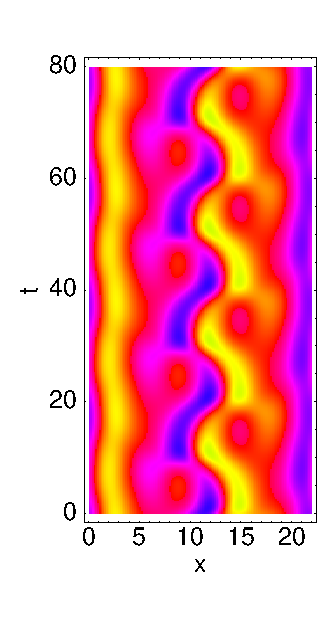
\includegraphics[width=0.2\textwidth]{../figs/rpoKS21}
(b)\includegraphics[width=0.2\textwidth]%,origin=c]
                {../figs/rpoKS33}
(c)\includegraphics[width=0.2\textwidth]%,origin=c]%
        {../figs/rpoKS46}
(d)\includegraphics[width=0.2\textwidth]%,origin=c]%
        {../figs/rpoKS56}
\end{center}
\caption[\Rpo s of KS equation]
        {
\Rpo s of KS
equation:
% for $\tilde{L}=3.5014$, N=64 mode truncation.
(a) T=20.51, d=0.0 (\po),
(b) T=32.80, d=10.96,
(c) T=46.51, d=7.76,
(d) T=55.60, d=-5.25.
        }
\end{figure}
%%%%%%%%%%%%%%%%%%%%%%%%%%%%%%%%%%%%%%%%%%%%%%%%%%%%%%%%%%%%%%%%%%

\PC{\refFig{f:KS22rpo} goes to Vaggelis thesis - removed it from the paper,
    as the color schme is different from Ruslan's
   }
It is imperative that we start using the discrete symmetries, and only 1/2
of trajectory when it is selfdual.
\EQV{1}, \EQV{2} and \EQV{3} and unstable eigenvectors
we care about all happen to sit in the antisymmetric subspace
(recheck...), so connections should reflect these multiplicities. We have
one $\EQV{2} \to \EQV{3}$ and $\EQV{2} \to \EQV{2}$ (shift by $L/4$).

The \rpo\ {\nameit}55 travels between the 2-\eqv\  and
2-\eqv\ shifted,
with period and shift
$\period{p}=55.5953\,,\ d=5.24725$
Compared to $L/4 = 5.5$
this is nice, but why not close to periodic after 2nd return? Why 4th return?

The {\nameit}2 {\eqv}
captures qualitatively the mean velocity frame \rpo\ {\nameit}55 shape,
which follows the
{\eqv} for most of the time, except for a quick swing where it
sidesteps by $d/4$, just as it does in \reffig{f:rpo55}.

\Rpo\ {\nameit}55 looks similar to Davidchack's  orbit
of period
$\period{p}=47.64$ and $d=5.6759$. The period appears to depend on how
many times the orbit manages to spiral around the \eqv.
For {\nameit}55 that appears to be
1.5 times per period, rather than 2. This would led as
to
think there is a family of \rpo s along with a 3rd unit eigenvalue of
$gJ$,
but such does not exist.
So there has to be a selection mechanism corresponding to
reaching or missing the neighborhood of an \eqv\  point starting from
the neighborhood of the other.

The $u$ space time evolution \reffig{f:rpo55u} % rpo22-55-4-u
is plotted with the same starting instant,
so one can also track also the spatial profile $u$ in parallel with
the Fourier space projections.

So it is almost impossible to see \reffig{f:rpo55}(b) %rpo22-55-4-cm
in \reffig{f:rpo55}(a) % rpo22-55-4.
I can see 4 periods in \reffig{f:rpo55}(a), %po22-55-4,
but not in \reffig{f:rpo55}(b) %rpo22-55-4-cm
where it comes back only after full period $\period{p}=55.6$.

It still seems that it could be made relative periodic
(modulo a reflection symmetry?)
in $\period{p}/4=55.6/4=13.9$? That would be OK
-
by symmetry the figure 8 connecting
2 symmetric {\eqva} could consist of 4 identical segments: from
{\eqv} A to midplane, then reflected version of the same to SA, and
back again.

The two {\eqva}
capture qualitatively the mean velocity frame \rpo\ {\nameit}55 shape,
which follows the
{\eqv} for most of the time, except for a quick swing where it
sidesteps by $d/4$, just as it does in \reffig{f:rpo55}.

Please also plot it in plane, chose small Fourier coefficients
 which respect the $x \to -x$ symmetry of \KSe.
Then the symmetry of 2 mean velocity
{\eqva} and self-dual symmetry of \rpo\ {\nameit}55 will be explicit.

Eigenvalues of \rpo\ {\nameit}55 $g\jMps$: are
\\
$(-57.17,  1, 1, -0.500, -0.012, \cdots)$ .
%
%  Eigenvalues of the Jacobian without rotation
%  84.15, -33.86 + 28.94 i, c.c. , 0.48, 0.00019
% no good - missing marginal ones

plots:
  76 rpo60fm23.jpg  \\
 909 rpo60fm23.emf  \\
% Ruslan L Davidchack,  10 Jul 2006
the 55 rpo, or whichever seems easiest to explain:
$\period{} = 59.89$,
$c_p = \shift_p/\period{p}= ?$

$(\ExpaEig_i e^{\pm i\theta_i})=
(
\\
 -27.03397007874626,
\\
   9.34426620337976,
\\
   1
\\
   1
\\
  -0.05018967056231,
\\
   0.00015065158255,
)$

The eigenvectors
indicate that an amplitude mode comes paired with the
group shift-invariant mode $\ExpaEig_4 =1$. It probably says that
the amplitude $|u_k|$ of the associated can be easily perturbed (think of
a large system: $|u(x)|$ can be easily deformed by long wavelength
perturbations. This \underline{must} be understood. Proposal:

There are two
marginal eigenvalues, one for time translation, one for
rotational invariance.
The sign of $\ExpaEig_{1}=-57$ says this is a Moebius-kind orbit,
inverse hyperbolic.
Stability exponent
 $\eigExp[1]=0.07$ says that this neighborhood is much less repelling than
the central {\eqv} A, a better candidate for being embedded into the
ergodic attractor.

The \rpo\ initial condition is
so accurate the orbit in \reffig{f:rpo55}(b)
start visibly deviating after retracing the loop 6.5 times.
% the largest unstable multiplier is
% $-57.17$ per period of the orbit - error would grow to $\approx 60^7
% = 2,800,000,000,000$.

For a numerical check of the \rpo\ stability eigenvalues,
used two inital
points along an unstable eigenvector $\jEigvec{1}$
at radial distance  $\approx 10^{-4}$ from the \eqv\ {\nameit}2,
and the initial inter-point separation $\Delta(0) \approx 10^{-5}$.
Integrated for time equal to the period $\period{p}=26.3556$ as calculated from
the \jacobianM\ and computed the leading Lyapunov exponent from the ratio of
final to initial distance
$\Lyap= \frac{1 }{ \period{}}\ln( \Delta(\period{})/\Delta(0))$.
Get
$\Delta(\period{})/\Delta(0) =39.01$,
$\Lyap=0.13902$, in agreement with the \eqv\ {\nameit}2
expanding eigenvalue $\Lyap=0.13904$
\[
\ExpaEig_{radial} =  e^{\Lyap \period{}} =38.99
\,.
\]

% Ruslan L Davidchack,  10 Jul 2006
The orbit RLD found has period 60
rather than 55.  Because it comes so close to the steady states,
this is probably a numerical precision error.
\\
plots:
 180 rpos1.jpg  \\
1594 rpos1.emf  \\


Rewrite Fourier modes as $u_k(t) = e^{r_k(t) + k(\theta_k(t))}$, study
dynamics and Jacobinas in the $\dot{r_k},\dot{\theta_k})$ representation.
\nameit 2 and \nameit 3 \eqva\ are nearly cirlces in this representation - higher
modes will not wind wildly if represented by $\theta_k(t)$? Kind of WKB
representation.

period 77 rpo jumps between the two steady states.
\\
plots:  \\
  84 rpo77fm23.jpg  \\
1133 rpo77fm23.emf  \\
 176 rpos2.jpg  \\
1594 rpos2.emf  \\


\bigskip

%%%%%%%%%%%%%%%%%%%%%%%%%%%%%%%%%%%%%%%%%%%%%%%%%%%%%%%%%%%%%%%%
\begin{figure}[t]
\begin{center}
(a) 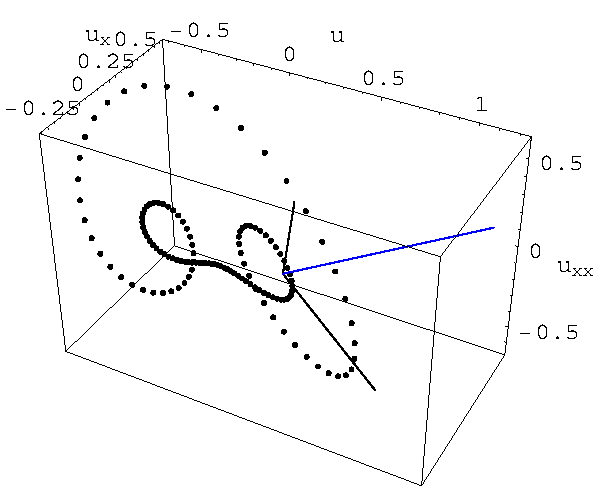
\includegraphics[width=5.0cm]{../figs/1wSteadyE}
\hspace{0.1in}
(b) 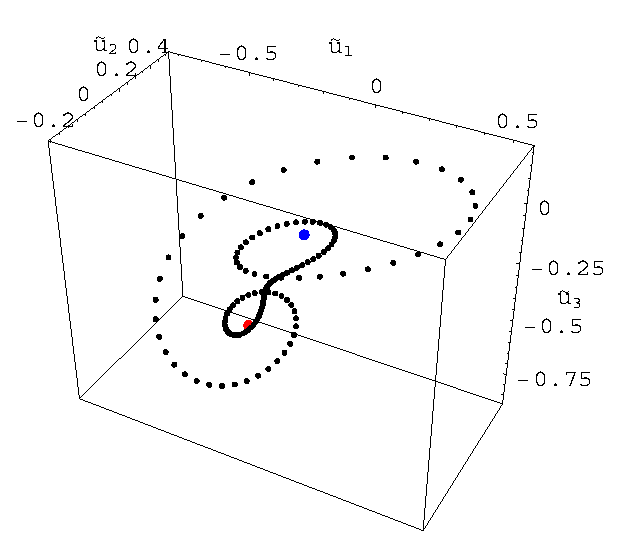
\includegraphics[width=5.0cm]{../figs/1wSteadyP}
\end{center}
\caption[EQV{1} visualization]
        {
(a) \EQV{1} in $(u,u_x,u_{xx})$ representation along with the eigenvectors of the equilibrium
point $(\sqrt{c},0,0)$. The blue line represents the unstable eigen-direction.
(b) \EQV{1} projected along the above eigenvectors.
% $\tildeL=3.5014$, $N=64$ complex modes truncation.
        }
\label{f:1wSteady}
\end{figure}


%%%%%%%%%%%%%%%%%%%%%%%%%%%%%%%%%%%%%%%%%%%%%%%%%%%%%%%%%%%%%%%%
\begin{figure}[t]
\begin{center}
    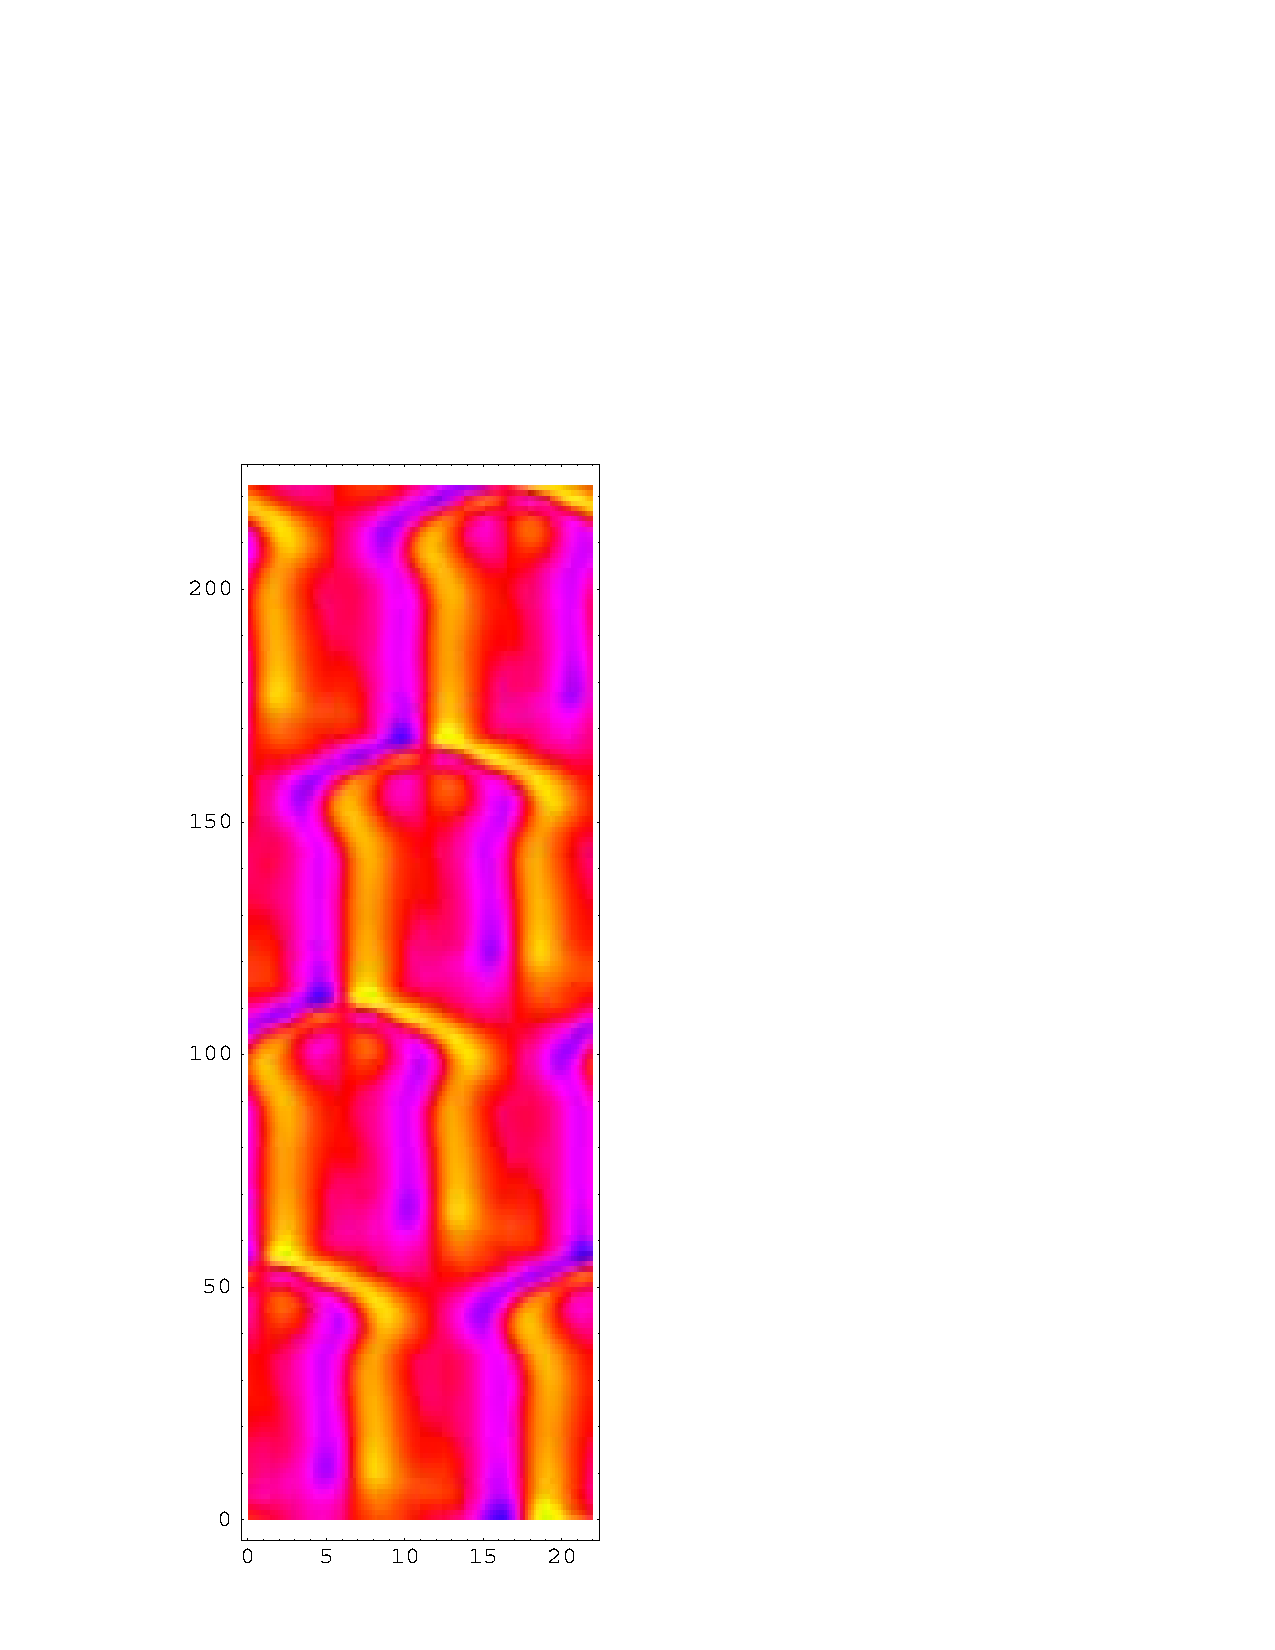
\includegraphics[width=0.18\textwidth]{../figs/rpo22-55-4-u}
\end{center}
\caption[The \rpo\ T=55 in  u(x,t)  representation]
        {
 The \rpo\ {\nameit}55 in $u(x,t)$ representation.
        }
\label{f:rpo55u}
\end{figure}
%%%%%%%%%%%%%%%%%%%%%%%%%%%%%%%%%%%%%%%%%%%%%%%%%%%%%%%%%%%%%%%%%%




This observation can be heuristically motivated as follows.
\PC{this argument keeps worrying me: there are lots of solutions, like
$u=0$, that are {\eqva}, but isolated -
they are noplace near asymptotic dynamics.
Do they belong to the invariant manifold?
   }
Equilibria are solutions valid for all times, and are thus points
on the finite-dimensional compact inertial manifold\rf{infdymnon}.
Finite dimensionality of the inertial manifold
bounds the size of Fourier components of all solutions.
This
compact inertial manifold and the dynamics on it can be
described by analytic functions of a finite number of Fourier modes.
\PC{explain the theory; say that in practice it is useless}
On a finite-dimensional compact manifold,
an analytic function can only have a finite number
of zeros. So the {\eqva}, {\ie},
the zeros of a smooth velocity field on
the inertial manifold, are finitely many.
The number of {\eqva} increases exponentially with $L$,
\PC{give reference for ``exponential growth''}
for infinite system size $L \to \infty$,
there are infinitely many {\eqva}.
\PC{is there a reference where this is explained?}

\bigskip

To illustrate the rapid contraction in the non-leading eigendirections
we plot  in [MAYBE INCLUDE] % \reffig{f:eigenvalues}
the eigenvalues of the \eqv\ in the unstable regime,
for relatively small system size, % low viscosity $\nu$,
and compare them with the
stability eigenvalues of the least unstable cycle for the same
system size.
The `laminar' \EQV{0}~\eqv\ is very unstable,
with many unstable eigendirections.


\bigskip

Even though our starting point \refeq{ks} is an infinite-dimensional
dynamical system, the asymptotic dynamics unfolds on a
finite-dimensional attracting manifold, and so we are back on the
familiar territory: the theory of a finite number of ODEs applies to
this infinite-dimensional PDE as well.

\bigskip

It is very unlikely that a single 1-$d$ Poincar\'e section,
can do the job, previous work\rf{Lan:Thesis,lanCvit07}
always needed several sections.

The idea is that the local unstable plane gives 2 coordinates, the
least contracting direction (or one of a complex pair) gives the 3rd.

We need to construct the backbone of heteroclinic connections
first. They are not like 3-$d$ R\"ossler and Lorenz examples:
here one spirals out,
then spirals in - hopefully there will be intelligent Poincar\'e sections
transverse to initial \EQV{2} (or {\EQV{3)} unstable manifold, mapping onto
Poincar\'e sections of trajectories leaving again
the next \EQV{3} or \EQV{2} unstable manifold.

% Ruslan:  10 Jul 2006
%
% 119 KB     "long_orbit.jpg"
% ----------------------------------------

For all spatial plots color axis $u \in [-3, 3]$ is the same,
same time units and spatial width $L$.
For the steady states the magnitude of the \EQV{2} is quite
a bit smaller than that of the \EQV{3}.

On the
    $[a_?,a_?]$ plane
    the $\sigma x = -x$ symmetry of \KSe\ is explicit.


As it looks, will not help us with partitioning, it seems, unless there is
a trajectory that hits the contracting direction - maybe
( -0.11941393,0)
head on.

Might want to look at this blowup in
the \EQV{2} slowest contraction
$   ( -0.08402656 \pm i 0.16019413)$
complex eigenvectors plane, check whether the
spiralling rotation agrees with the real/imaginary parts of eigenvalues.

Question is still - why does all of the unstable manifold of
\EQV{2}~\eqv\ go back
into
\EQV{2}~\eqv?


\underline{1-\reqv\  (traveling wave).}
% Ruslan L Davidchack,  10 Jul 2006
There is a pair of {\reqva}
${\nameit}1L$,
${\nameit}1R$
(traveling waves), dual under the
$u(x) \to -u(-x)$ symmetry. They are
determined numerically by
adiabatic continuation from a smaller system size
$L~\approx 12$,
where they are stable, to $L=22$
where their velocity is atypically large, $c=0.737$,

Their exponents are:
\\
$\Lyap_i \pm \theta_i =
(
\\
  0.1156222 \pm 0.817289,   \\
  0.033663 \pm 0.418909,    \\
 0.0                    ,   \\
 -0.245729                    , \\
 -0.321321 \pm 0.98126,
\cdots
)$

{\bf PC}:
Plot also the two \eqva\ of \eqva\ points, their
real eigenvectors and their complex eigenplanes. All {\eqva} presumably
wind around these, and as box size $L$ changes, they form continuous
families with smoothly changing $E$. One can check that by
changing $L$ a bit and using the previous \eqv\ to find the next
one.

What does the complex eigenplane continuation does for these
{\eqva} - does it produce nice heteroclinic connections, or is it
weirder? We know there is an analytic formula for a heteroclinic
connection (see \refref{Lan:Thesis}). % Lan's thesis).

Linearization of the flow around $C_{+}$ yields the cubic equation
  \beq
\eigExp(1+\eigExp^2) = 4 \expctE
  \ee{flot:KSeqvCubic}
for the
stability eigenvalues
$\eigExp[j] = \eigRe[j] \pm i \eigIm[j]$.
% of \refeq{KSeqvStab}.
They can
be given in any of the standard analytical forms for cubic
roots  (all useless in practice), such as
\beq
[ 2\eigRe \,, -\eigRe \pm i \eigIm ]
    \,,\qquad
\eigRe=\frac{1}{\sqrt{3}}\sinh \phi
\,,\qquad
\eigIm=\cosh \phi \, ,
\ee{flot:eqvEqvEigV}
with $\phi$ fixed by $\sinh 3\phi=3\sqrt{6\expctE}$.

The pair of \reqva\
${\nameit}2L$,
${\nameit}2R$
exists for larger system sizes, but does not continue
adiabatically\rf{KNSks90} down to $L=22$.

%\PC{
%   (a) Vaggelis May version of \reffig{f:KS22EkEigs} is illegible
%when printed in B\&W. Also squeeshing $\Im \lambda$ (use
%$\eigExp[j]= \eigRe[j] \pm i\eigIm[j]$ notation) axis does not help.
%Restore the better proportions of the previous figure, return the
%list of dots back into the frame, but without a box around them.
% restore the previous, April version?  not important... %
% (b) do include  \EQV{0}.
%   (c) Again, make sure the colored points can be distinguished in B\&W.
%   }
% With $S$, $A$ we denote an eigenvector belonging to the symmetric
% or antisymmetric subspace respectively. The last column lists
% the symmetry expected to be present in the corresponding
% stable/ustable manifold.

% \PCedit{I suggest moving \reftab{tab:EkEigs} and related into Appendix,
% replacing them with figures like Gibson's
% \reffig{f:KS22EkEigs}.
%    }

{\bf RLD}:
I've used the same \KSe\ convention as Kassam and Trefethen.
If you google 'Kuramoto-Sivashinsky',
http://mathworld.wolfram.com/Kuramoto-SivashinskyEquation.html is
the first in the search list and it uses the same convention
(actually, their $u$ is actually a $w$ such that $w_x$ is my $u$.)
The site refers to a 1986 Physica D paper by Michelson and a
``Handbook of differential equations" by Zwillinger, but I haven't
seen either of these.

\noindent {\bf When is an \eqv\ important? a bit of speculation}
%
There are two kinds of roles
{\eqva} play:
(1)
a {\em `hole' in the natural measure}.
The more unstable eigendirections an \eqv\ has (for example, the
$u=$const \eqv~\EQV{0}), the more unlikely it is  that
an orbit will recur in its neighborhood.
(2)
{\em Unstable manifolds of the `least unstable' {\eqva}}.
Empirically, asymptotic dynamics tends to spend
a large fraction of time in
neighborhoods of a few  {\eqva} with
a least number of unstable eigendirections.




\section{Numerical searches for \reqva\ and \rpo s}

% \subsection{Newton's method for determining \reqva}


The problem one faces with high-dimensional flows is
that their topology is hard to
visualize, and that even with a decent starting guess for a point on
a periodic orbit, standard methods like Newton-Raphson are likely to fail.
Methods that start with initial guesses for a number of points along the
cycle, such as the multi-point shooting methods,
% of \refsect{s-MultShoot},
are more robust.

  Our first task is to determine all \eqva\
and  \reqva\ of the \KS\ system for a given fixed domain size
$L$.
This problem is equivalent to
finding periodic orbits of a 3-$d$ ODE system \refeq{eq:3dks} together
with determining appropriate value of the integration constant $E$.
In \refrefs{CvitLanCrete02,lanVar1,Lan:Thesis,lanCvit07} they are
determined by a variational {\descent} method; for {\eqva} determined here,
straight Newton method sufficed.

% In the current investigation
%we prefer to search for \eqv\ solutions in
% the Fourier space
% \ beq
%  \dot{b}_k=\dot{c}_k=0
% \,.
% \eeq
% This is inefficient comapred to the above 3-$d$ ODE methods, but
% it serves as a warmup for, and the first test of methods that we then use
% to locate \po s and \rpo s.

%  Expanding $\dot{b}_k(a)$ and $\dot{c}_k(a)$ around our initial guess $a_o$ and demanding that they satisfy the equilibrium
%  condition, we get
%  \bea
%   \dot{b}_k(a) & = & \dot{b}_k(a_o)+\left.\frac{\partial \dot{b}_k}{\partial b_j}\right|_{a_o}\delta b_j + \left.\frac{\partial \dot{b}_k}{\partial c_j}\right|_{a_o}\delta c_j = 0 \continue
%   \dot{c}_k(a) & = & \dot{c}_k(a_o)+\left.\frac{\partial \dot{c}_k}{\partial b_j}\right|_{a_o}\delta b_j + \left.\frac{\partial \dot{c}_k}{\partial c_j}\right|_{a_o}\delta c_j = 0
%  \eea
%  or in matrix form
%  \beq
%     \left( \begin{array}{cc}
%         \frac{\partial \dot{b}}{\partial b} & \frac{\partial \dot{b}}{\partial c} \\
%         \frac{\partial \dot{c}}{\partial b}   & \frac{\partial \dot{c}}{\partial c}
%      \end{array}
%      \right)_{a_o}
%      \left(\begin{array}{c}
%        \delta b  \\
%        \delta c
%      \end{array}\right)
%      =
%      \left(\begin{array}{c}
%        -\dot{b}(a_o) \\
%        -\dot{c}(a_o)
%      \end{array}\right)\,,
%      \label{eq:NewtonEquil}
% \eeq

%% ES Sep 11 2006 Commented out PC text. Added appendix with details of
%% Calculations to answer JFG question of Sep 7 2006.
%PC incorporated JFG Sep 7 2006 remark:
% Additional computational savings can be achieved
% for the \KS\ solutions that are restricted
% to the antisymmetric subspace of \refsect{s:AntisymmSubsp}.
% For the 3-$d$ ODE periodic solution this symmetry reduces
% the length of the loop by factor $1/2$. In the Fourier representation
% the continuous translation symmetry is eliminated by
% setting  the coefficients to purely imaginary values $i a_k$,
% thus reducing the dimensionality of the (truncated) \statesp\
% by factor 2. In fluid dynamics such savings are very significant,
% and are enforced whenever possible; for small cell \KS\ systems
% studied here they are not so important, and we search for such
% \eqva\ in the full space, and use the size of the (symmetry violating)
% real Fourier coefficients as an
% additional test of the accuracy of our Newton searches.

{\bf PC}: STUDY - this suggests that \expctE\ grows with system size:
   The last type of solution identified in \refref{ksgreene88}
   appears at point $F$  in the original reffig~{fig:GreeneKim}
   and is called a
   `giant' state because its amplitude grows as the system size
   increases.



{\bf PC}: bit weird: can use Galilean invariance to
    set $\expctE=0$ for any given $u(x,t)$?


{\bf ES}:  We can, but this effectively
sets $a_0$ to some value. The rate of change of energy depends only on the
non-zero modes only and thus the value of energy will not remain zero. I don't
see any problem with this.
}

{\bf RLD}: But it's the same as with kinetic energy, which is zero
in the reference frame that is moving with the object. Right?

% JFG Sep 7 2006: Do you then
% enforce real-valuedness in your Newton-descent via the constraint
% $a_{-k} = a^*{k}$ (the conjugates that then appear in the equations
% are nondifferentiable which is a big pain) or do you let the solutions
% go complex and then choose the real part at the end?
% The cost of that
% is that the dimension of your search space is twice as big as it needs
% to be. That's an unacceptable cost in fluids; perhaps in \KS\ it's not.
% In any case, I think you should (1) either clarify that you're no
% longer working in the antisymmetric subspace or eliminate its mention
% earlier, and (2) explain how you ultimately arrive at real-valued
% solutions.


\subsection{Bridges says:}

p.j. aston SIAM J Math Anal. in 1990 - first showed how the sequence of bifurcating branches
are related to each other by the scaling symmetry of KS

John Elgin and Wu did all this hook orbit stuff, bottleneck orbits, followup on
\refref{kskent92}

perturbations with respect to $L$ are modulational instabilities, or Eckhaus  instabilities

For example, the energy of \reqva\ \REQV{\pm}{2} which
seems close to the
mean turbulent energy in \reffig{f:drivedrag} is separated
from it when plotted along the
$\expct{u \, u_{x}{}^2}$ moment, where according to
\refeq{Bridges1} it takes nonzero value $c P$.

\subsection{Eigenvalues for high $k$}

We need to include  \EQV{0}
in \reffig{f:KS22EkEigs} and similar figures, because
PC believes that for larger $k$ all solutions have the same eigenvalues. This
    would enable us to separate dynamical from "hyper-diffusion" spectra,
    tell us how many are dynamically significant. This is different from Navier-
Stokes,
    which has zillion contracting complex eigenvalue pairs.

\subsection{Computing energy from Fourier modes}
The energy of $u(x)$ is defined as
\[
   E = \frac{1}{L}\int_0^L \textstyle\frac{1}{2}u^2(x) dx
\]
In terms of Fourier modes
\[
   E = \sum_{k=-\infty}^\infty {\textstyle\frac{1}{2}}|a_k|^2 =
   \sum_{k=1}^\infty |a_k|^2
\]

-----------------

    \PCedit{still to be incorporated, most likely in the next paper:
    wrote down \refeq{KSD1} in order to (a) to clarify embedding of
    $\bbU^+$ into $\bbU$
    (b) to explain the desymmetrization of evolution defined on
     $\Omega^{+} = [0, L/2]$ fundamental domain, with evolution at
    instant of crossing $x=0$ given by reflection $\Refl$.
    Re integrators: make sure $\Refl$ applied after
    all points used by integrator are in $\bbU^-$
    }

    \PCedit{abandoned the \refref{KNSks90} notation, I might be wrong,
        please recheck. Replace $\mathbf{L} \to P^{(1)}$ downstream}

\bigskip

 Integrate over $L$, and $u_x$, $u_{xx}$ drop put by the
  $L$ periodicity.
 Written as a ,
\refeq{eq:stdks}
 this is a volume preserving flow
 % \beq
 % \ESedit{
 % v = u_x \,,\qquad
 % w = v_x \,,\qquad
 % w_x = \expctE - {\textstyle\frac{1}{2}} u^2 + c u - v
 %        }% end ESedit
 % \,,
 % \label{eq:3dks}
 % \eeq
 \ES{
 Changed signs here, seemed simpler this way.
 PC: I remember having a reason, so something down the line
     came out with consistent signs. Perhaps \refeq{eqvOfEqv}?
    }
 with the `time' reversal symmetry,
 \[
 x \to -x,\quad u \to -u, \quad v \to v, \quad w \to -w \,.
 \]
     \ES{
    The term $c u$ breaks the symmetry.
    We may overcome this by changing sign of c as well,
    but it is a parameter, not a variable.
        }
 \PC{might move space average def \refeq{rpo:spac_ave} to here,
     note that
     $\expct{u} = \expct{v} = \expct{w} =0$
     }
  Rewriting \refeq{eq:3dks} as
      \ES{With the corrected form of \refeq{eq:stdks} we cannot write this}
 \beq
 \PCedit{
 (u+w)_x={\textstyle\frac{1}{2}}(u-c)^2-\expctE
     ={\textstyle\frac{1}{2}}(u-c-\sqrt{2\expctE}) (u-c+\sqrt{2\expctE})
        } %end \PCedit{
 \ee{eqvOfEqv}
 we see that
 for $\expctE<0$,
     \ES{Isn't $E>0$ by definition?
     PC: Here $E$ is an integration constant - do not see how
     we can argue $E \geq 0$ at this point.
         }
 $u+w$ increases without bound with $x \to \infty$,
 and every solution escapes to infinity.
 If $\expctE=0$, the origin $(0,0,0)$ is the
 only bounded  solution, a marginally stable center with
% eigenvalues $(0, i,-i)$.

\bigskip

\ES{Removed text about equilibria of equilibria.}
% ES removed
%%%%%%%%%%%%%%%%%%%%%%%%%%%%%%%%%%%%%%%%%%%%%%%%%%%%%%5
 The solutions of the {\eqv}  condition
 \refeq{eq:3dks} are
 % themselves in turn
 organized\rf{Mks86} by the
 `{\eqva}  of {\eqva}'  condition
 \( u_x= v_x= w_x= 0 \).
 % , and the connections between them.
     For $\expctE>0$ the {\reqva}  points of \refeq{eqvOfEqv} are
 $C_{+}=(c+\sqrt{2\expctE},0,0)$ and $C_{-}=(c-\sqrt{2\expctE},0,0)$.
 Linearization of the flow around $C_{+}$ yields the cubic equation
 $ %  \beq
 \eigExp(1+\eigExp^2) = 4 \expctE
 \,,
 $ %  \ee{KSeqvCubic}
 with linear stability eigenvalues
 \beq
 \eigExp[1] = 2 \eigRe
     \,,\qquad
 \eigExp[2,3] = - \eigRe \pm i \eigIm
 \ee{eqvEqvEigV}
 Hence $C_{+}$ has a {1\dmn}
 unstable manifold and a 2\dmn\ stable manifold
 along which solutions spiral in.
 By the $x \to -x$ `time reversal' symmetry, the
 invariant manifolds of $C_{-}$
 have reversed stability properties.
 \PC{
     not sure we need this, not used in our paper? Where did the figure go?
     }
 Most orbits escape quickly even if initiated close to \eqva, and that
 renders the numerical calculations
 difficult\rf{ksham95,kshooper88,pimyk,pimsimp}.
 In this context the variational method
 developed in \refrefs{lanVar1,CvitLanCrete02}
 appears more robust than
 the earlier approaches.

\begin{table}[t]
\caption[Experimental layout of \reftab{tab:Eksym}]{
\PCedit{Experimental layout of \reftab{tab:Eksym} symmetries
        (incomplete, just testing the layout).
Need a rational way to label symmetries. The main thing we care about is
whether eigenvector is in $\bbU^-$, in which case its global continuation
remains within $\bbU^-$.
        }
        }\label{tab:EksymTEMP}
\begin{center} \footnotesize
\begin{tabular}{lccccc}
      && $\eigRe[j]$ & $\eigIm[j]$ & ~~~\Refl & $\Shift_{1/2}$\\
\EQV{2}&& &  & \\\hline
 &$\eigExp[1,2]$ & $~0.1390$ & $0.2384$ & $\Refl_1$         & $\bbU^-$\\
 &$\eigExp[3]$   & $0$      &          & $\Shift_{1/2}$        & $\Shift_{1/2}$\\
 &$\eigExp[4,5]$ &$-0.0840$ & $0.1602$ & $\bbU^-$           & $\Refl_1$\\
 &$\eigExp[6]$   &$-0.1194$ &          & $\Shift_{1/2}$        & $\Shift_{1/2}$\\
 &$\eigExp[7,8]$ &$-0.2711$ & $0.3563$ & $\Refl_1,\,\bbU^-,\,\Shift_{1/2}$  & $\Refl_1,\,\bbU^-,\,\Shift_{1/2}$\\
 &$\eigExp[9]$   &$-2.0130$ &          & $\bbU^-$           & $\Refl_1$\\
 &$\eigExp[10]$  &$-2.0378$ &          & $\Refl_1$         & $\bbU^-$\\
\EQV{3}&&  &  & \\\hline
 &$\eigExp[1]$   &$~0.0933$  &          & $\Refl_1$     & $\bbU^-$\\
 &$\eigExp[2]$   &$~0.0933$  &          & -         & -  \\
 &$\eigExp[3]$   &$0$       &          & $\Shift_{1/3}$    & $\Shift_{1/3}$\\
 &$\eigExp[4]$   &$-0.4128$ &          & $\Refl_1,\,\Shift_{1/3}$  & $\bbU^-,\,\Shift_{1/3}$\\
 &$\eigExp[5,6]$ &$-0.6108$ & $0.3759$ & $\Refl_1$     & $\bbU^-$\\
 &$\eigExp[7,8]$ &$-0.6108$ & $0.3759$ & -         & -\\
\end{tabular}
\end{center}
\end{table}

PC{ dropped this:
    ``The eigenvectors do not belong to any of the symmetric
    subspaces of {\KSe} discussed in \refsect{sec:KSeSymm}."
    }

ES{ dropped: We use these dynamically invariant solutions
as a scaffolding from which to explore the
\statesp\  topology and chaotic dynamics.
}%end ES

ES{ dropped:  While in general
for $\tildeL$ sufficiently large
one expects many
coexisting attractors in the \statesp%
%Hyman and Nicolaenko
\rf{HNZks86},
in numerical studies most random initial
conditions converge to the same chaotic attractor.
}%end ES


%\PC{please list $c$ in \reftab{tab:TW} }
%\begin{table} \label{tab:TW}
%\caption{
%Stability eigenvalues of the \reqva\ for $L=22$.
%} %\ for $L=22$.}
%\begin{center} \footnotesize
%\begin{tabular}{ccc|ccc}
%  \multicolumn{3}{c}{$\REQV{\pm}{1}$ ~($c = \pm 0.73699$)}  &
%  \multicolumn{3}{c}{$\REQV{\pm}{2}$ ~($c = \pm 0.34954$)} \\\hline
%  &$\eigRe[j]$ & $\eigIm[j]$ & & $\eigRe[j]$ & $\eigIm[j]$\\
%  $\eigExp[1,2]$ & $0.1156$ & $0.8173$ & $\eigExp[1]  $ & $0.3370$ & \\
%  $\eigExp[3,4]$ & $0.0337$ & $0.4189$ & $\eigExp[2]  $ & $0$ & \\
%  $\eigExp[5]$   & $0$      &          & $\eigExp[3,4]$ &$-0.0096$ & $0.6288$\\
%  $\eigExp[6]$   &$-0.2457$ &          & $\eigExp[5,6]$ &$-0.2619$ & $0.5591$\\
%  $\eigExp[7,8]$ &$-0.3213$ & $0.9813$ & $\eigExp[7,8]$ &$-0.3067$ & $0.0725$\\
%\end{tabular}
%\end{center}
%\end{table}


%%%%%%%%%%%%%%%%%%%%%%%%%%%%%%%%%
% end ES removed

%\subsection{\Eqva\ on a periodic domain}
%

% \begin{table}[t]\label{tab:EkEigs}
% \begin{center} \footnotesize
% \caption{ Eigenvalues of the \eqva\ for $L=22$.}
% \begin{tabular}{cccc} \hline
%   \EQV{0}  &    \EQV{1}        &    \EQV{2}        &  \EQV{3}   \\\hline
%   $0.2198$ &  $0.1308+i0.3341$ &  $0.1390+i0.2384$ &  $0.0933$\\
%   $0.2198$ &  $0.1308-i0.3341$ &  $0.1390-i0.2384$ &  $0.0933$\\
%   $0.1952$ &  $0.0824+i0.3402$ &  $0$              &  $0$\\
%   $0.1952$ &  $0.0824-i0.3402$ & $-0.0840+i0.1602$ & $-0.4128$\\
%   $0.0749$ &  $0$              & $-0.0840-i0.1602$ & $-0.6108+i0.3759$\\
%   $0.0749$ & $-0.2287+i0.1963$ & $-0.1194$         & $-0.6108-i0.3759$\\
%  $-0.3981$ & $-0.2287-i0.1963$ & $-0.2711+i0.3563$ & $-0.6108+i0.3759$\\
%  $-0.3981$ & $-0.2455$         & $-0.2711-i0.3563$ & $-0.6108-i0.3759$\\
%  $-2.1191$ & $-2.0554$         & $-2.0130$         & $-1.6641$\\
%  $-2.1191$ & $-2.0619$         & $-2.0378$         & $-1.6641$\\\hline
% \end{tabular}
% \end{center}
% \end{table}


---------------------

    \PC{
        are there
        {\bf (c)} \po s which have $D_m$ symmetries?
        }

 Spatial representations of PDEs (such as the 3$D$
 snapshots of velocity and vorticity fields in Navier-Stokes)
 offer little insight into detailed dynamics of low-$Re$ flows.
 Much more illuminating are the \statesp\ representations.
 \PC{expand this into a visualization subsection: how we use
     $d$-dimensional vectors (stability eigenvectors, etc) to project
     from $d$-dimensions to 2 or 3 dimensions. \underline{Not}
     Fourier modes as coordinates!}

\PC{Check next what these 2 unstable eigenvectors for \EQV{3}~\eqv\ are
    - when they are equal in magnitude you expect a `star',
    all directions in their plane going straight out.
    Do they all fall into \EQV{2}~\eqv?
    }


% relativeKS.tex
% copied here from nsf/nsf06am/TEX/relativeKS.tex       Nov 1 2006
%%%%%%%%%%%%%%%%%%%%%%%%%%%%%%%%%%%%%%%%%%%%%%%%%%%%%%%%%%%%%%%%%%
\PC{
    if there is something useful in this paragraph, incorporate into the
    text, the rest of this file goes to flotsam.tx.
    }
In \reffig{f:KS22unstM} the \eqv~\EQV{1} of
\reffig{f:KS22unstM}(a) is represented by the point~\EQV{1},
and its unstable manifold can be examined in great detail.
To each \eqv\ point corresponds a continuous family
of \eqva, and this leads to an unexpected feature of such
flows: While in dimensions higher than 2 heteroclinic connections
are a rarity (likelihood that unstable manifold of one
 \eqv\ precisely hits another \eqv\ point is zero),
for flows with continuous symmetries intersections of unstable
manifolds with continuous families of equivalent \eqva\ are common.
\refFigToFig{f:KS22E1man2}{f:KS22E3man} show
such heteroclinic connections.
% from an $\EQV{2}$~\eqv\ point to $\EQV{3}$~\eqv\ family.
These connections offer an invariant partition of the \statesp.
%,and will be the basis of our
%{construction of symbolic dynamics}.

\RLDedit{We expect that the number of \po s with
symmetry (b) and period $\period{}$ should be similar to the number
of \rpo s with period $\period{}/2$.  The reason is that, provided
the dynamics is equally mixing for all types of orbits,
it should be equally possible to match $-u(-x+d,\period{}/2)$
and $u(x,0)$, as it is to match $u(x+d,\period{})$ and $u(x,0)$,
especially for larger $\period{}$.  So far, we have found 51 \po s
with $\period{} < 200$ and 78 \rpo s with $\shift > 0$ and
period $\period{} < 100$.}
\RLD{What do you think about this paragraph?  Can we include it in
the paper?}
 \RLD{ It looks like there
 might be many more \po s than I initially expected to find. In fact, I
 can even venture a guess that there are approximately as many \po s
 with symmetry (2) within $\period{} < 200$ as there are \rpo s within $\period{} <
 100$. The reasoning is that it shouldn't be any harder to match
 $-u(-x+d,\period{}/2)$ and $u(x,0)$, than it is to match $u(x+d,\period{})$ and
 $u(x,0)$, provided the dynamics is equally mixing for all types of
 orbits.  If this is true, then the number of \po s with period smaller
 than $\period{}/2$ should be approximately equal to the number of \rpo s with
 period smaller than $\period{}$; the equality improving with increasing
 $\period{}$.
     }

, indicating non-hyperbolicity of the
chaotic attractor through unstable dimension
variability\rf{kostelich97}.
[Ref.???\RLD{Maybe give reference to one of the classical papers on UDV, for example,
 R. Abraham and S. Smale, Proc. Symp. Pure Math. {\bf 14}, 5 (1970),
 or  S. P. Dawson, C. Grebogi, T. Sauer, and J. A. Yorke, Phys. Rev.
 Lett. {\bf 73}, 1927 (1994)}].

    \PC{
    do not like notation $s_j$ for `Lyapunov exponent' but
    let it be, for now...
    }

 % \subsection{\Reqva}
 \PC{
     \refTab{tab:Eksym}:
     replace D(m) by $\tau_{1/m}$  (?),
     \\
     $A(L/4)\EQV{n}$ symmetry by $\tau_{1/4}\EQV{n}$ (?)
     \\
     link caption to equations in symmetry section
    }
 In addition to the \eqva, the KS system has pairs of
 \reqva\ \refeq{reqva} with fixed profiles
 moving at constant speed $\pm c$, \ie,
 \PCedit{ $u(x - ct,t)$, so they travel to the right for $c>0$ }
 \[
 u(x \PCedit{-} ct,t) = u(x, 0)\,.
 % \quad t \in \mathbb{R}\,.
 \]

%\begin{figure}[t]
%\begin{center}
%%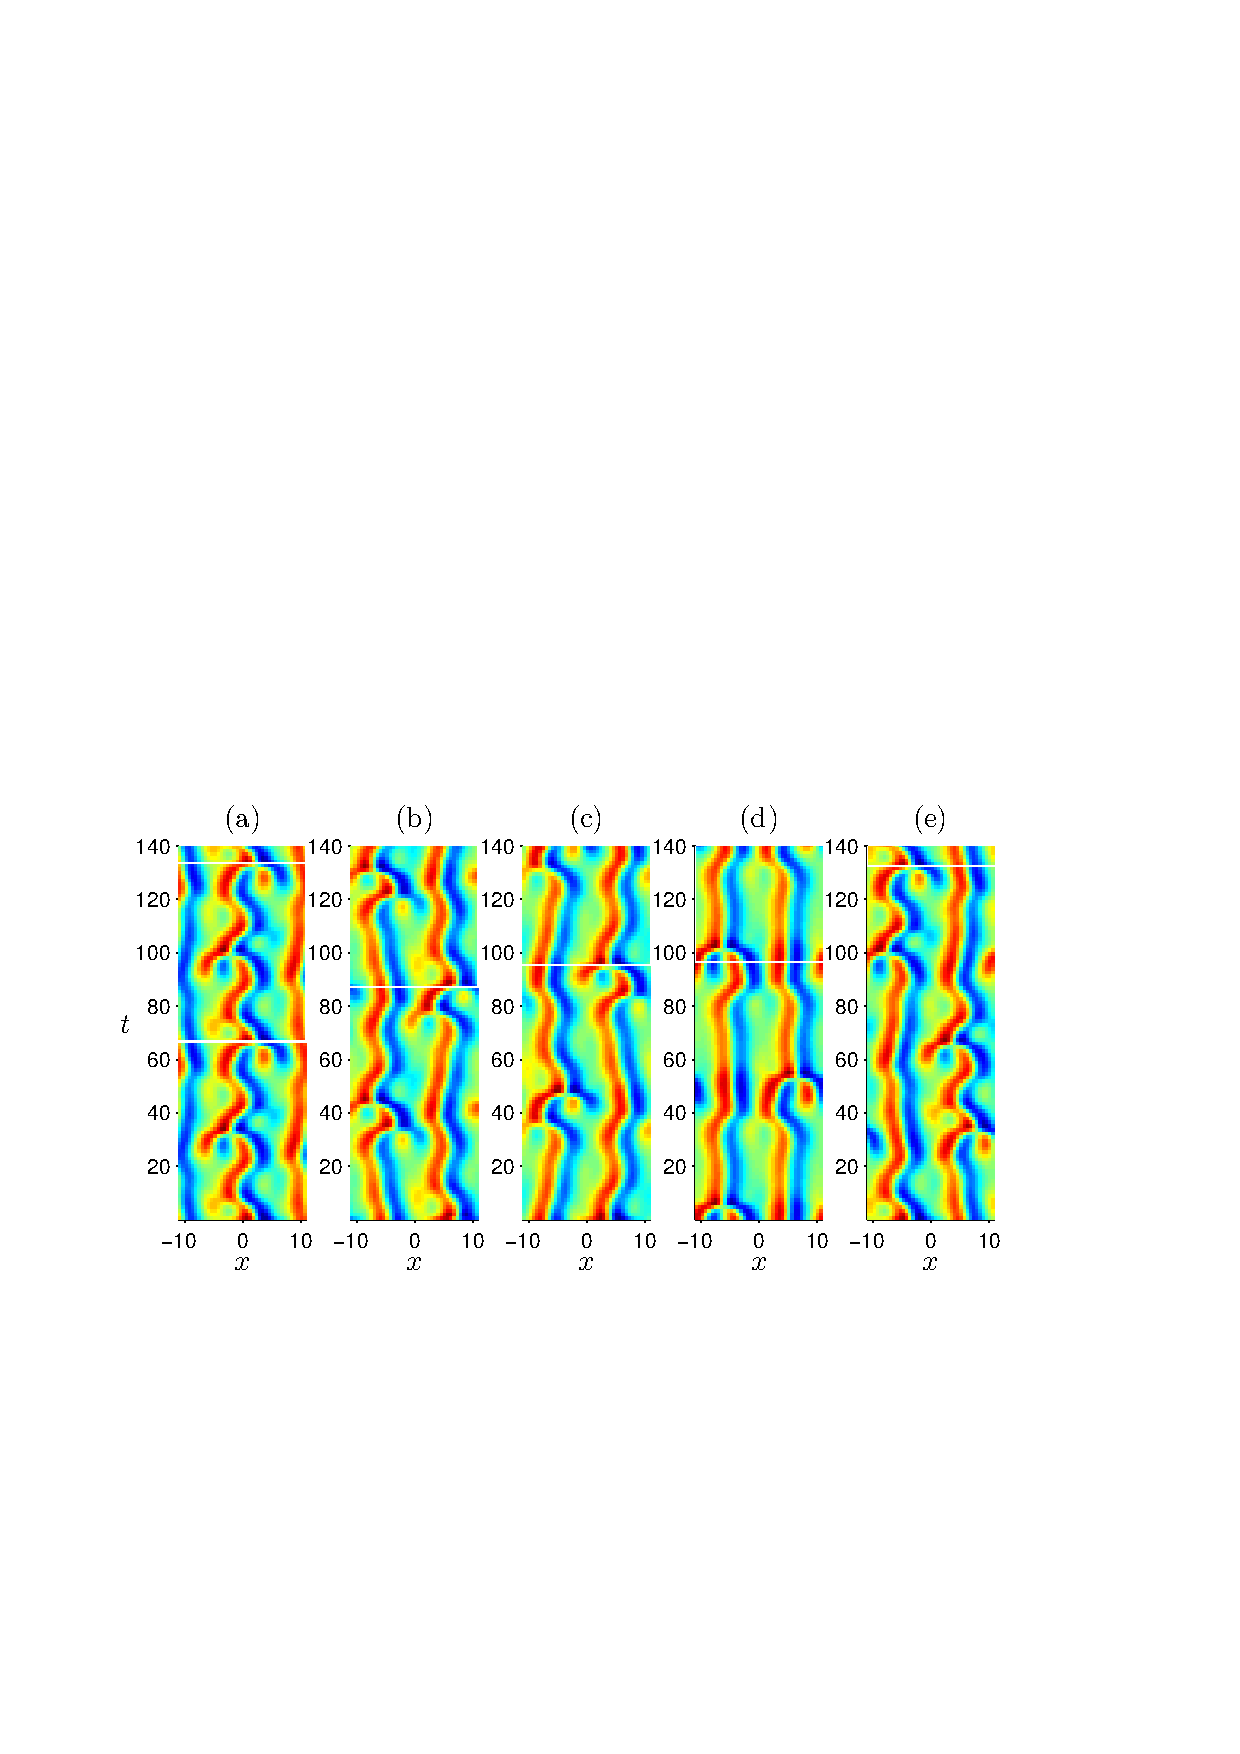
\includegraphics[width=0.9\textwidth]{figs/ks22rposPO}
%\begin{tabular}{ccccc} (a) & (b) & (c) & (d) & (e)\\
%$t$
%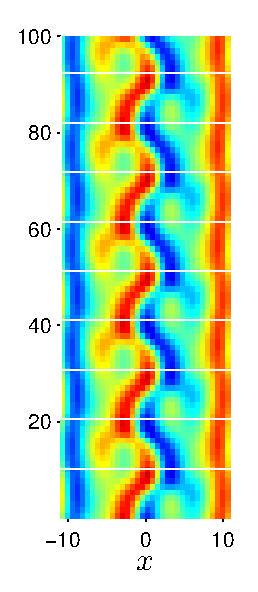
\includegraphics[width=0.18\textwidth]{figs/ks22rpo020.5-00.00}\hspace{-3ex} &
%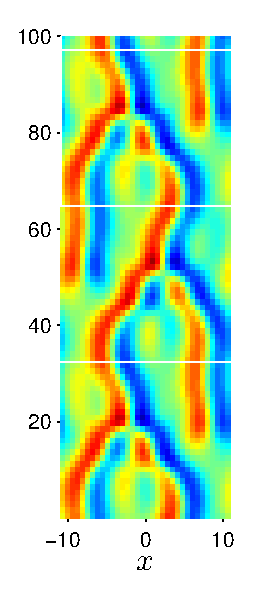
\includegraphics[width=0.18\textwidth]{figs/ks22rpo064.7-00.00}\hspace{-3ex} &
%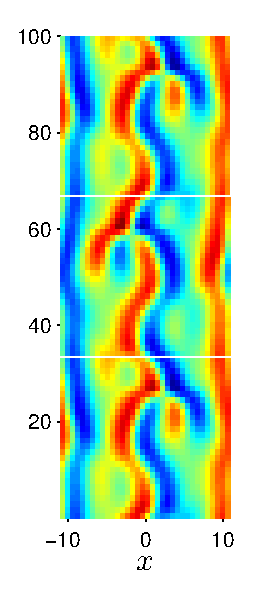
\includegraphics[width=0.18\textwidth]{figs/ks22rpo066.8-00.00}\hspace{-3ex} &
%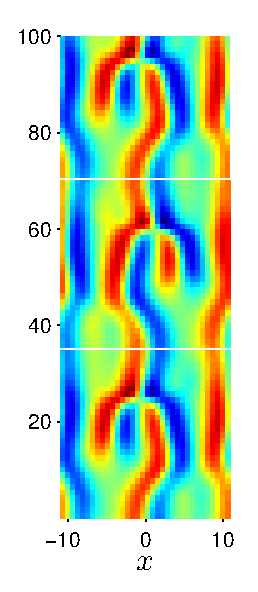
\includegraphics[width=0.18\textwidth]{figs/ks22rpo070.3-00.00}\hspace{-3ex} &
%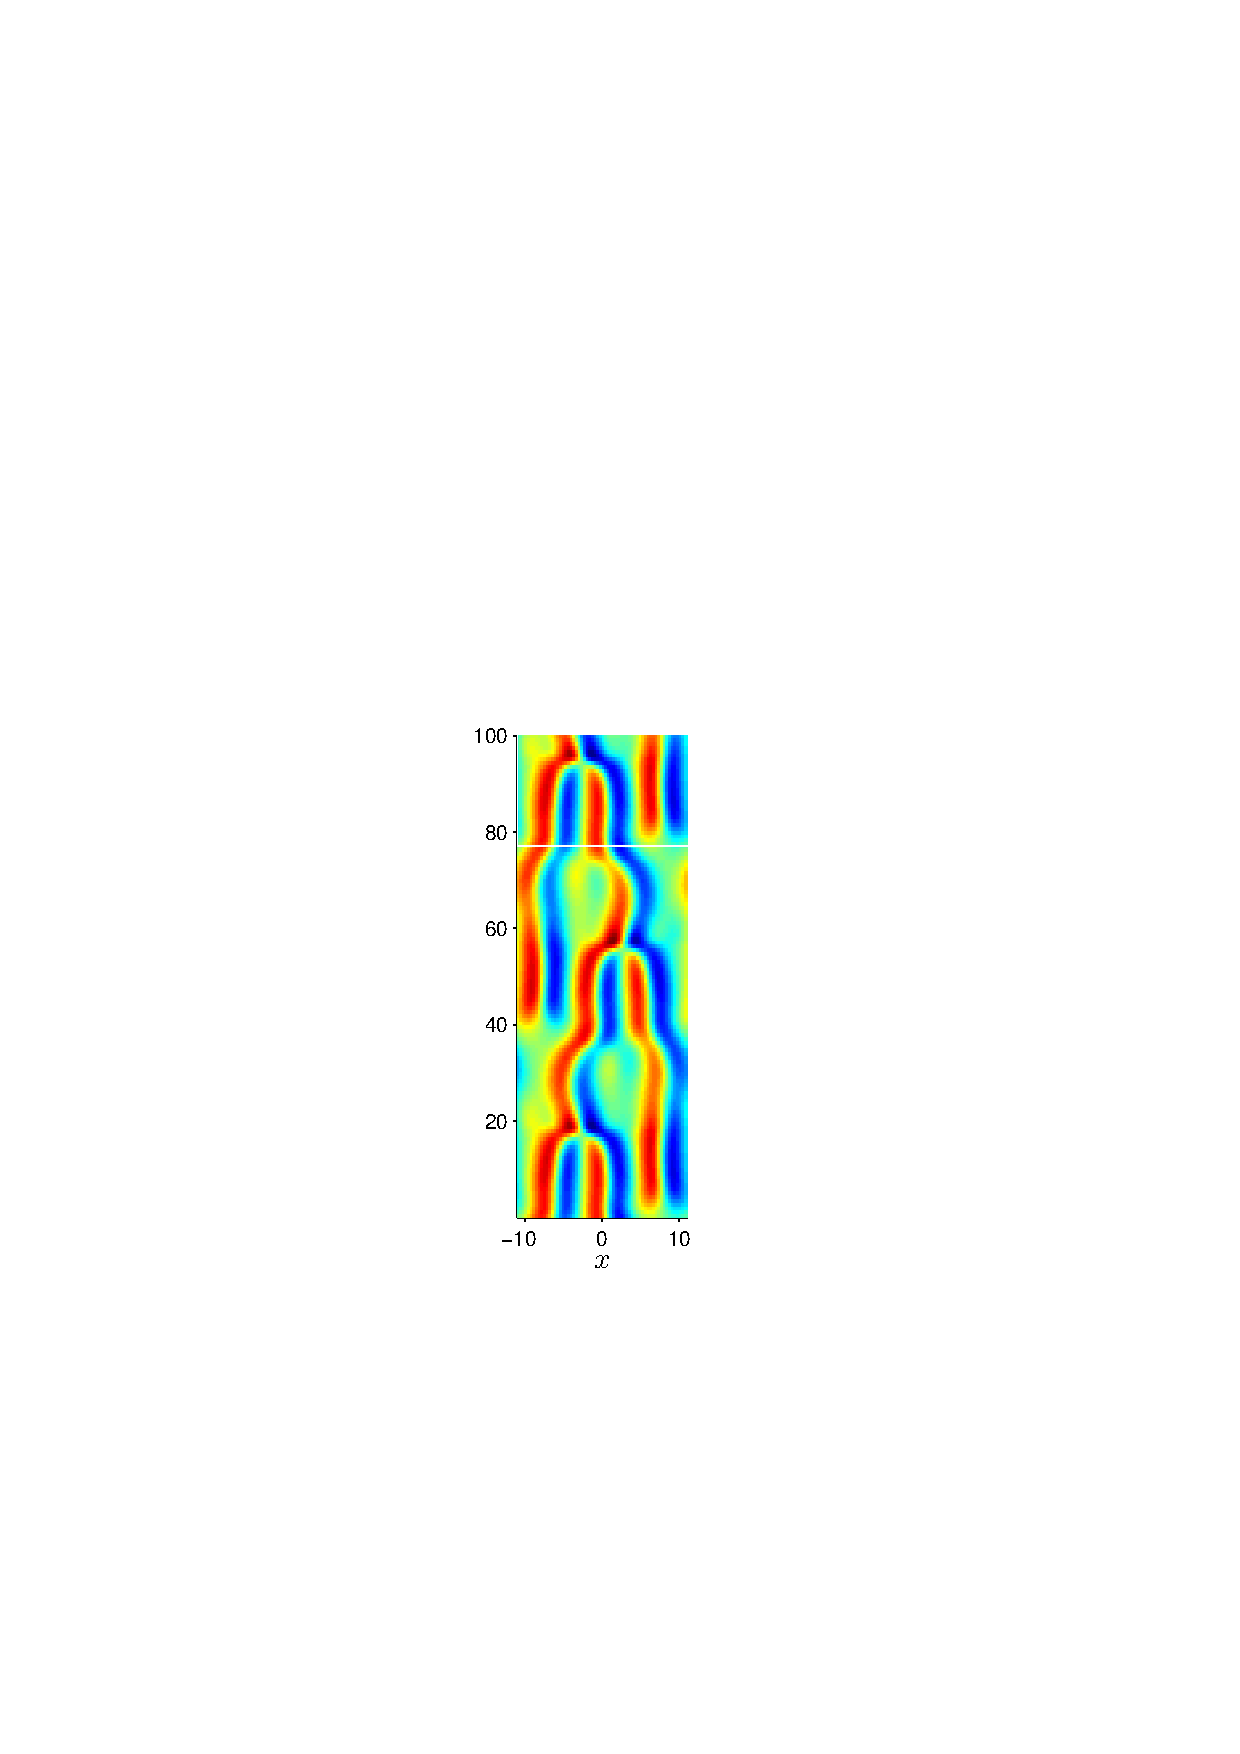
\includegraphics[width=0.18\textwidth]{figs/ks22rpo077.2-00.00}
%\end{tabular}
%\end{center}
%\caption{\Po s of \KS\ equation with $L = 22$:
%(a) $\period{} = 20.5$;
%(b) $\period{} = 64.7$;
%(a) $\period{} = 66.8$;
%(b) $\period{} = 70.3$;
%(c) $\period{} = 77.2$.} \label{f:ks22rposPO}

%\begin{figure}[t]
%\begin{center}
%%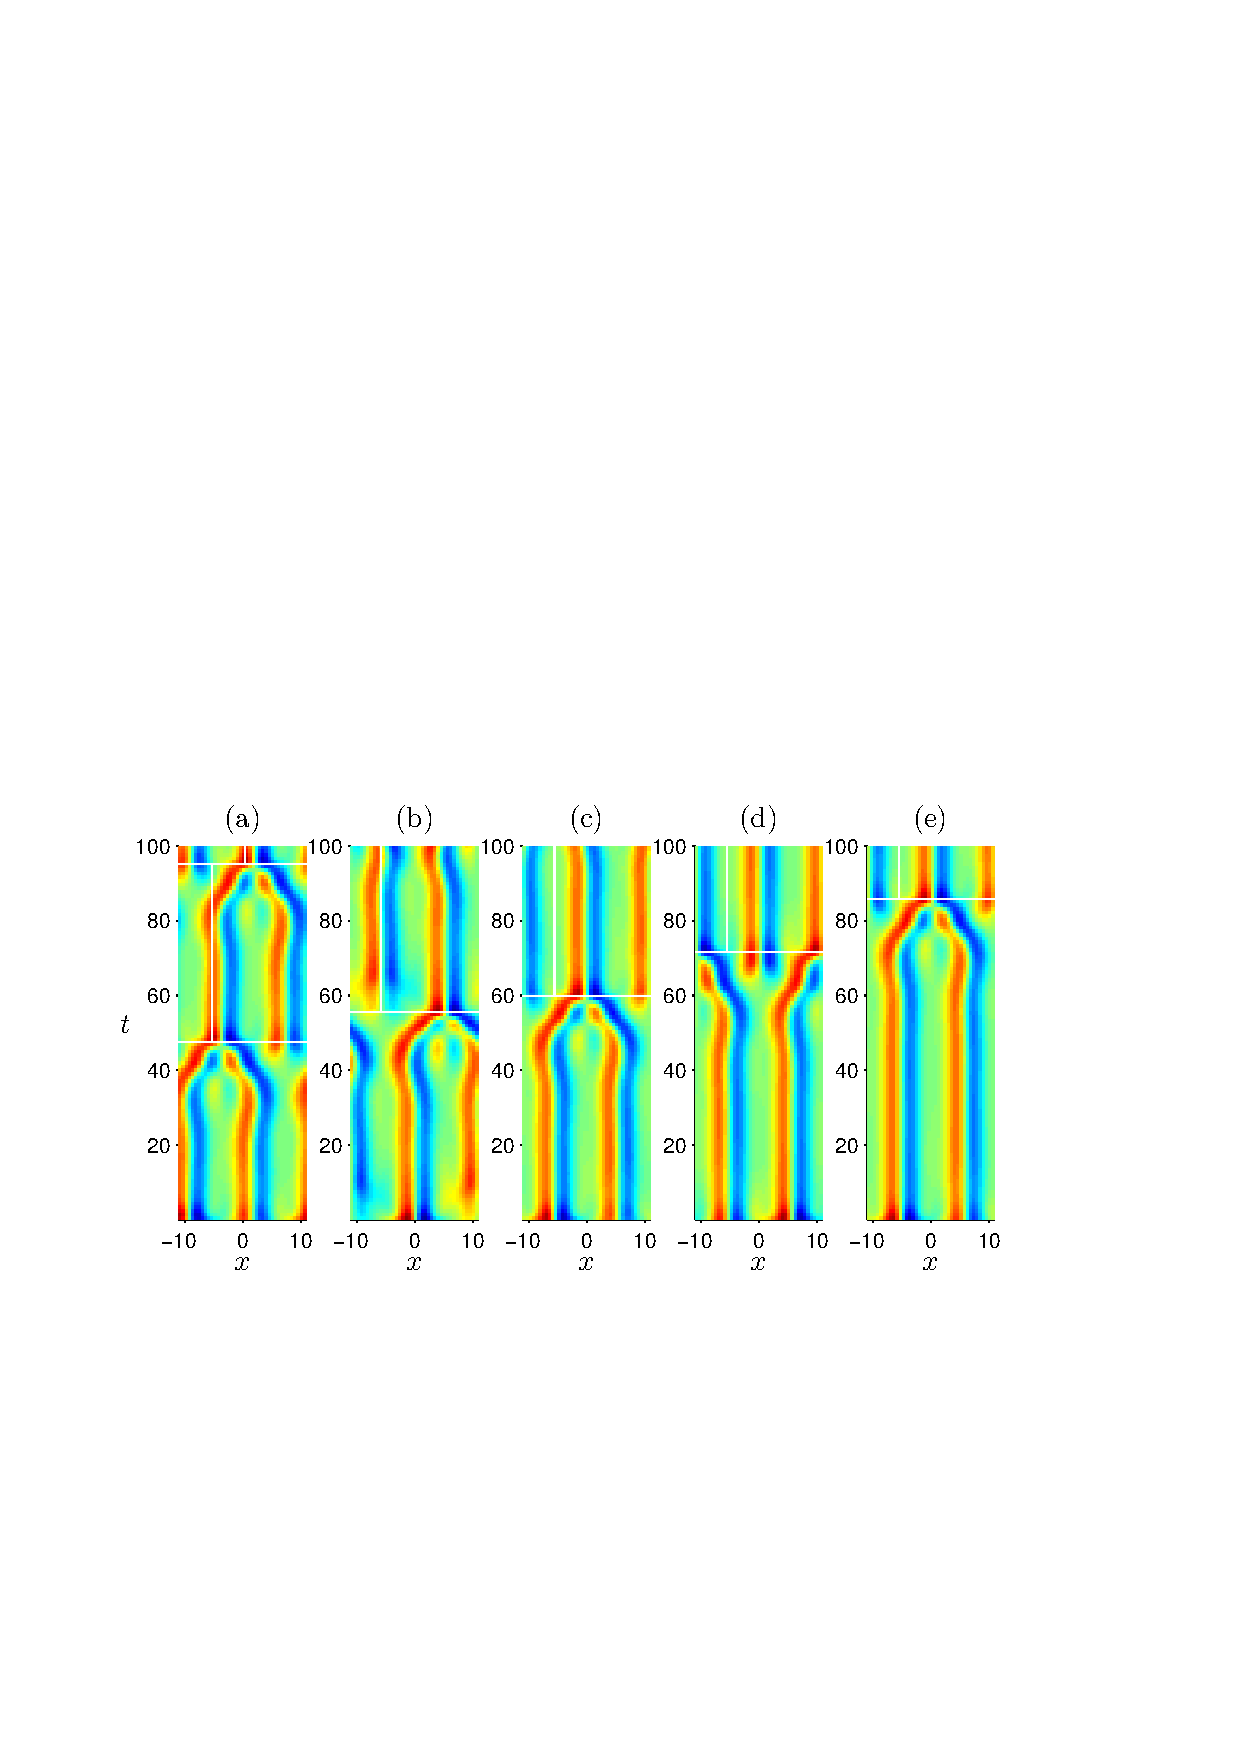
\includegraphics[width=0.9\textwidth]{figs/ks22rposCage}
%\begin{tabular}{ccccc} (a) & (b) & (c) & (d) & (e)\\
%$t$
%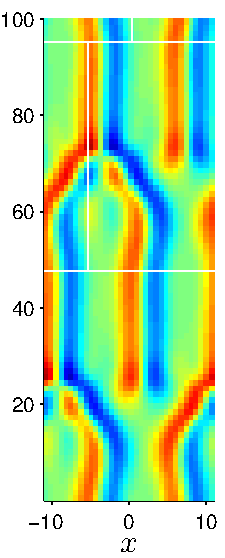
\includegraphics[width=0.18\textwidth]{figs/ks22rpo047.6-05.68}\hspace{-3ex} &
%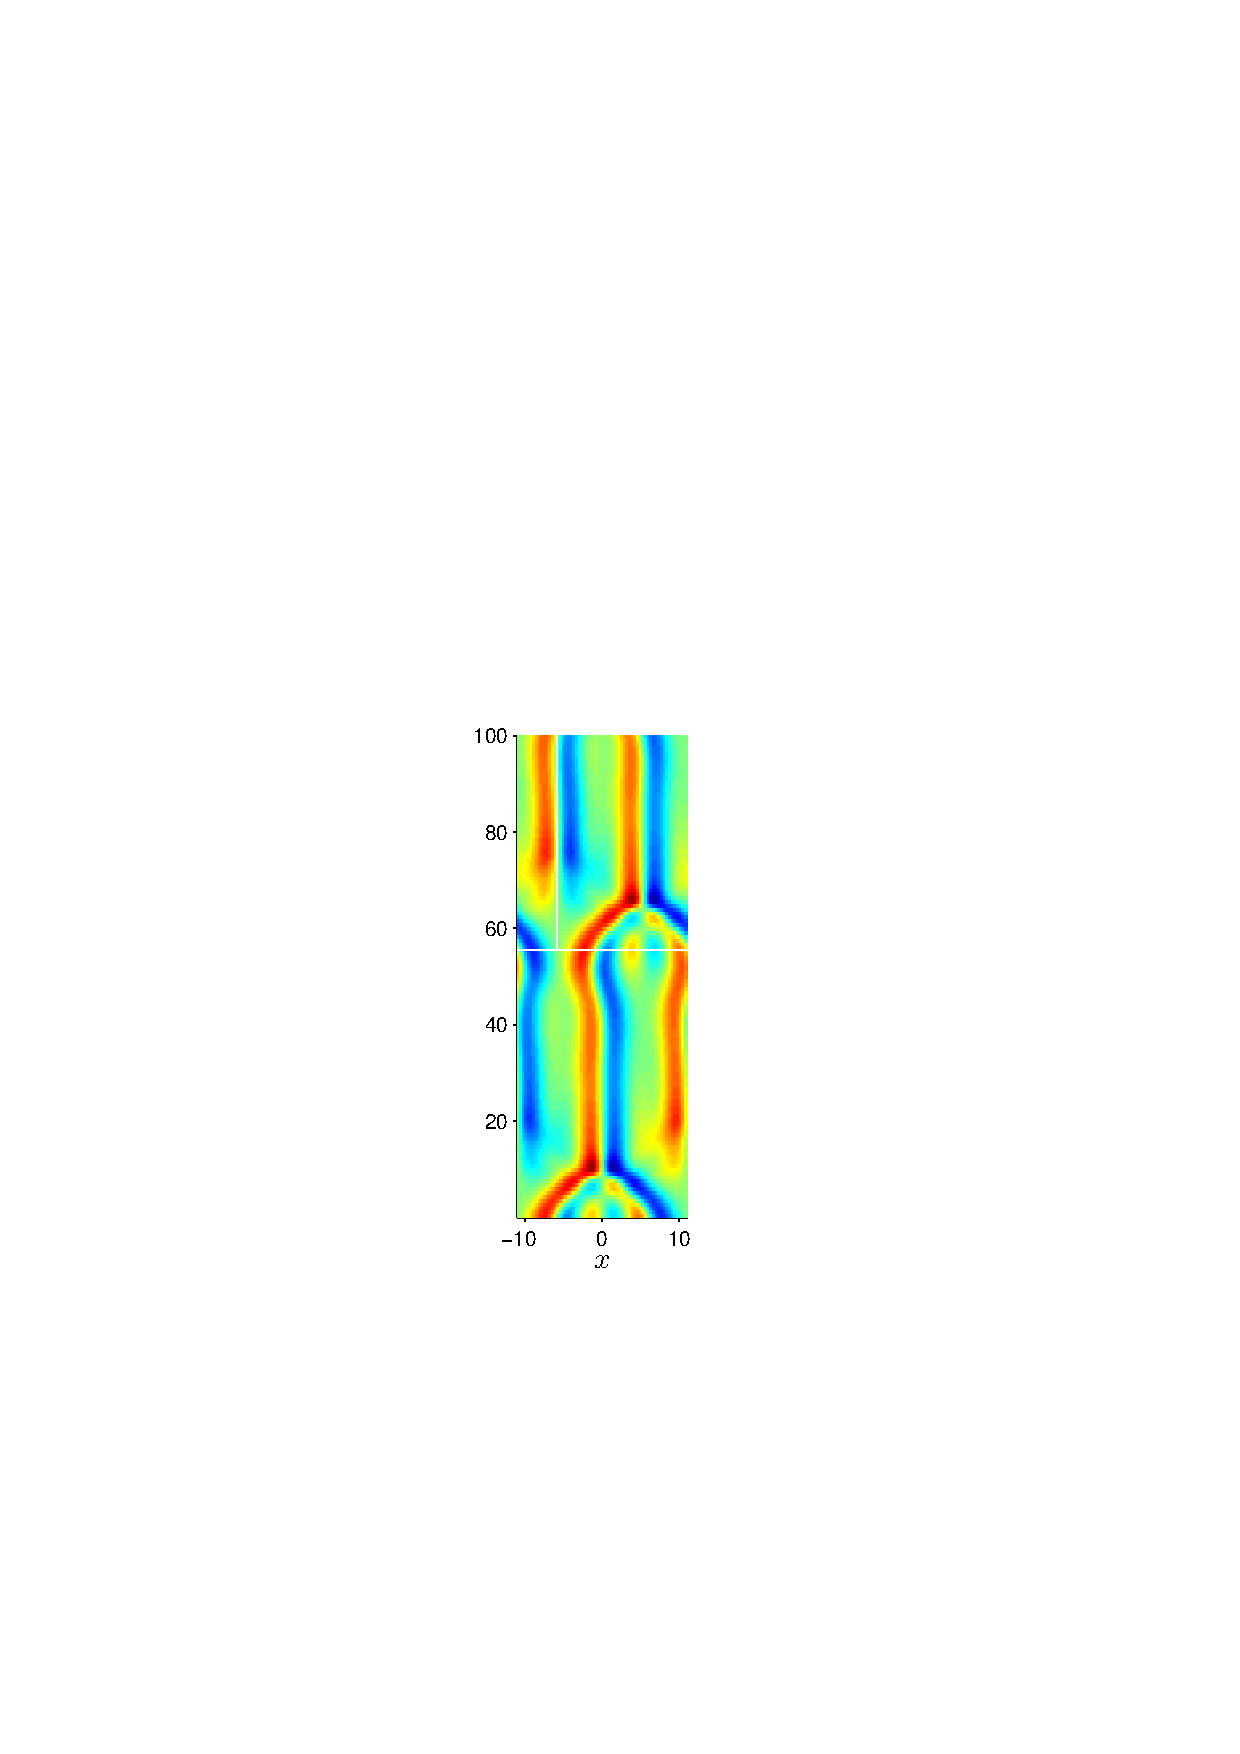
\includegraphics[width=0.18\textwidth]{figs/ks22rpo055.6-05.25}\hspace{-3ex} &
%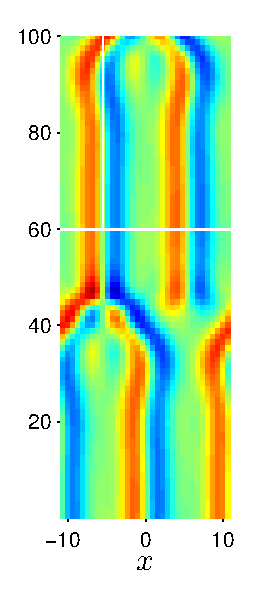
\includegraphics[width=0.18\textwidth]{figs/ks22rpo059.9-05.44}\hspace{-3ex} &
%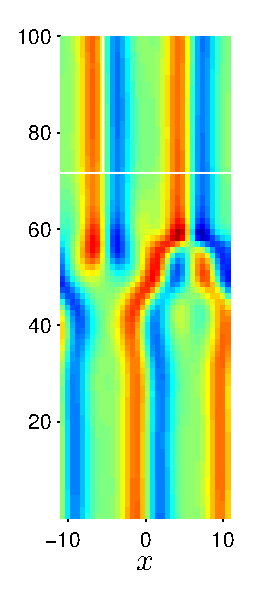
\includegraphics[width=0.18\textwidth]{figs/ks22rpo071.7-05.50}\hspace{-3ex} &
%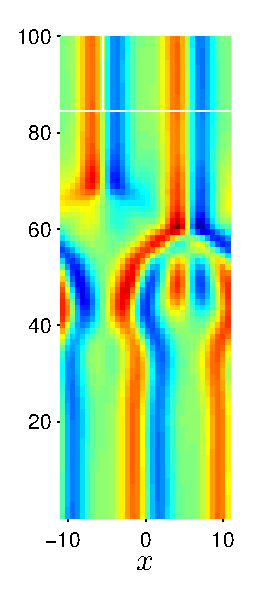
\includegraphics[width=0.18\textwidth]{figs/ks22rpo084.4-05.51}
%\end{tabular}
%\end{center}
%\caption{\Rpo s close to the unstable manifold of \EQV{2} equilibrium.
%(a) $\period{} = 47.6$, $\shift = 5.68$;
%(b) $\period{} = 55.6$, $\shift = 5.25$;
%(c) $\period{} = 59.9$, $\shift = 5.44$;
%(d) $\period{} = 71.7$, $\shift = 5.503$;
%(e) $\period{} = 84.4$, $\shift = 5.513$.
%Horizontal and vertical white lines indicate periodicity and
%phase shift of the orbits, respectively. }\label{f:ks22rposCage}
%\end{figure}

%    \RLD{
%    \RLDedit{I've split the \reffig{f:ks22rposShort}
%plots and put them in the tabular,
%but I don't know how to place label $t$ to the left of the figures.
%Please fix this if you know how.  Otherwise I can include $t$ in the
%leftmost figure, but it will be a bit tricky since the aspect
%ratio of this figure will be different from the others.
%    }}
% \subsection{\Rpo s close to the unstable manifold of \EQV{2} }

% \PC{
%  Implementing Ruslan: all axes in \reffig{f:drivedragConn} changed by a factor
% of 2?
%         \\
% Implementing Predrag:
% label axes in \reffig{f:drivedrag}, \reffig{f:drivedragConn}
% by $(E,P,D,\dot{E})$
%     }
% \PC{ks22TurbConn2\_xfig for \reffig{f:drivedragConn}
%     not checked in?
%    }
% \PC{\refFig{f:drivedragConn}: split into three figures, \\
%     (a) label axes $(E,P)$, move to \reffig{f:drivedrag}\,(\textit{b})\\
%     (b) flip $y$ axis as $\dot{E}=P-D$; label axes $(P,\dot{E})$ \\
%     (c) flip $y$ axis; label axes $(E,\dot{E})$ \\
%    }

\medskip

RLD:{Replaced text: ``
As a result, KS equation can have
\rpo\ solutions with a profile $u_p(x)$, period $\period{p}$, and a
nonzero shift $\shift_p$, without or with reflection,
\begin{eqnarray}
  \Shift_{\shift_p/L}u(x,\period{p}) &=&
  u(x+\shift_p,\period{p}) = u(x,0) = u_p(x)\,,
\label{KSrpos0} \\
  \mbox{or} \quad \Refl\Shift_{\shift_p/L} u(x,\period{p}) &=&
  -u(-x-\shift_p,\period{p}) = u(x,0) = u_p(x)\,,
\label{KSpos0}
\end{eqnarray}
\ie, a profile $u(x,0) = u_p(x)$ that occurs again after time
$\period{p}$, but shifted by $\shift_p$, and possibly reflected by
$\Refl$.
   ''}
\RLD{
As a result, KS equation can have \rpo\ solutions with
a profile $u_p(x)$, period $\period{p}$, and a
nonzero shift $\shift_p$
\beq
  \Shift_{\shift_p/L}u(x+\shift,\period{p}) =
  u(x+\shift_p+\shift,\period{p}) = u(x+\shift,0) = u_p(x)\,,
\eeq
as well as \rpo s \emph{with reflection} which are characterized by
a profile $u_p(x)$ and a period $\period{p}$ and satisfy
the condition
\beq
  \Refl u(x+\shift,\period{p}) =
  -u(-x-\shift,\period{p}) = u(x+\shift,0) = u_p(x)
\label{KSpos1}
\eeq
with any $-L/2 < \shift \leq L/2$.
   } %end RLD

ES:{ I think we don't need the extra $\shift$. In the case with no reflection
the shift is uniquelly determined. In the case with reflection, since the term \rpo\
refers to the action of any group element under which the flow is invariant (not
necessarily translations) we can define this type of \rpo\ through
\[
  \Refl u(x,\period{p}) =
  -u(-x,\period{p}) = u(x,0) = u_p(x)\,.
\]
The \rpo s related to the action of $\Refl\Shift_{\shift/L}$ are equivalent (by translation) to
the last case (this is what Ruslan's footnote in \refsect{sec:L22} shows). Thus
there is no notion of shift associated with preperiodic orbits.
} %end ES

RLD:{
The reason I've introduced arbitrary $\shift$ is that this allows
the definition of the whole family of equivalent orbits related
by $\Shift_{\shift/L}$.  I agree with Vaggelis that, in case of RPOs
without reflection, it makes no difference, since the condition
\refeq{KSrpos} remains true in any spatial reference frame.  So we could
drop $\shift$ here.

However, in the case of POs (aka RPOs with reflection),
removing $\shift$ makes the condition \refeq{KSpos} valid only in
a specific reference frame, which is different for different POs.
Hence the condition as written in \refeq{KSpos} cannot be used to
find POs (i.e., you cannot derive \refeq{KSposFour} from it).

Now, if we don't use $\shift$ in \refeq{KSrpos}, but use it in \refeq{KSpos}
(like in \refeq{KSpos1}), then the two definitions are not equivalent,
since \refeq{KSrpos} defines just one orbit from the family related
by $\Shift_{\shift/L}$, while \refeq{KSpos1} defines the whole family.
   } %end RLD

ES:{ We can derive \refeq{KSposFour} by reversing Ruslan's proof:
applying $\Shift_{\shift/L}$ on \refeq{KSpos} we get
 $\Refl\Shift_{-2\shift/L}\left(\Shift_{\shift/L}u(x,T)\right)=\Shift_{\shift/L}u(x,0)\,,$
a condition for a \rpo\ of type \refeq{KSpos} in the translated frame, from which we get
\refeq{KSposFour}, to be used in practice since our initial guess might be translated
to another frame of reference.
The argument is that orbits of type \refeq{KSrpos} and \refeq{KSpos}
exist and are unique up to translational invariance.
We then can present the complications due to
translational invariance in their determination separately.
} %end ES


RLD:{
    The shift $\shift_p$ cannot be defined
    uniquely for a given pre-periodic orbit.  Let's say
    $\Refl\Shift_{\shift_p/L} u(x,\period{p}) = u(x,0)$.  The same
    orbit translated by any $\shift$ satisfies the condition
    $\Shift_{\shift/L}\Refl\Shift_{\shift_p/L} u(x,\period{p}) =
    \Shift_{\shift/L}u(x,0)$, or, since $\Shift_{\shift/L}\Refl = \Refl\Shift_{-\shift/L}$,
    this can be rewritten as follows:
    $\Refl\Shift_{(\shift_p - \shift)/L}u(x,\period{p}) =
    \Refl\Shift_{(\shift_p - 2\shift)/L}[\Shift_{\shift/L}u(x,\period{p})] =
    \Shift_{\shift/L}u(x,0)$, and so the new shift is now $\shift_p - 2\shift$.  Therefore
    $\shift_p$ can have any value depending on the spatial reference frame.  For example,
    we can always find a reference frame where $\shift_p = 0$ and thus the pre-periodic
    orbit satisfies the condition $u(x,\period{p}) = -u(-x,0)$.
    }

PC: check out @refref{szendro-2007} (and references therein)
    on uses of Lyapunov vectors in spatiotemporal chaos.

More references on "Lyapunov modes", this time in Hamiltonian setting, are in
 arXiv:0709.3143 (pick up BibTeX entry there)
``Lyapunov Mode Dynamics in Hard-Disk Systems"
D. J. Robinson, G. P. Morriss
